% !TEX root = ../main.tex

% 实验记录	
\begin{table}
	\renewcommand\arraystretch{1.7}
	\centering
	\begin{tabularx}{\textwidth}{|X|X|X|X|}
		\hline
		Major： & Physics & Grade： & 2022 \\
		\hline
		Name： & 杨舒云 & Student number： & 22344020\\
		\hline
		Room temperature： & 20\degree C & Experimental location： & A101 \\
		\hline
		Student Signature：& \textbf{In Attachment} & Score： &\\
		\hline
		Experiment time：& 2024/12/20 & Teacher's Signature：&\\
		\hline
	\end{tabularx}
\end{table}
\section{APL1-2 Vacuum Compatibility Testing of Materials and Plasma Characteristics Study \\ Experimental Record}


%---------------------------------------------------------------------
% 实验过程记录
\subsection{Content, Procedures \& Results}

% 操作步骤
\subsubsection{Operations}
\begin{enumerate}
	\item 使用机械泵和分子泵获得高真空。 
	\begin{enumerate}
		\item 启动机械泵观察记录真空度（真空计压强） 随时间（5 分钟） 的变化。 机械泵先
		抽真空压强低于 10 Pa 后， 启动分子泵观察记录真空度（ 真空计压强） 随时间的变
		化， 待分子泵达到额定转速（约需 8 分钟） 后再观察记录（5 分钟） 。
		\item 停止分子泵观察记录真空度（真空计压强） 随时间的变化（分子泵转速降为零约
		需 8 分钟） 。 待分子泵完全停止后， 关闭机械泵， 记录真空度（真空计压强） 随时
		间的变化（5 分钟） 。
	\end{enumerate}
	
	实验结果如\cref{fig:apl12exp1down}和\cref{fig:apl12exp1up}所示。
	
	\item 通过真空气体放电实验， 测量击穿电压与电极间隙和气压之间的关系， 验证帕邢定律， 了解气体放电基本物理过程。
	\begin{enumerate}
		\item 检查实验设备：
		\begin{itemize}
			\item 测量电极间实际间距。
			\item 确保放电管与电源连接可靠，电压和气体流量旋钮均调至最小位置。
			\item 确保高压电源开关和分子泵电源开关处于断开状态。
		\end{itemize}
		\item 打开总电源，启动机械泵，抽真空至 2-3 Pa（约 10 分钟）。
		\item 调节减压阀，使流量计前气压保持在 0-1 个大气压（由指导教师操作）。
		\item 调节流量计，使放电管内气压稳定在 20 Pa，记录真空计读数。
		\item 打开高压电源开关，逐步升高电压：
		\begin{itemize}
			\item 快速升至 200 V，再缓慢升高直至气体击穿，记录击穿电压及对应气压。
			\item 缓慢降压至 0 V，观察放电熄灭电压，并注意与击穿电压的差异。
		\end{itemize}
		\item 调整气压并重复测量：
		\begin{itemize}
			\item 增加气体流量，每次升高气压至 30 Pa、40 Pa、...、100 Pa，重复击穿电压测量（共 8 组数据）。
			\item 减小气压至 20 Pa，重复击穿测量。
			\item 逐步减小气压，每次减少约 2 Pa，直至 4 Pa，重复测量（共 7-8 组数据）。
		\end{itemize}
		\item 实验结束：
		\begin{itemize}
			\item 将气体流量和电压调至最小值。
			\item 依次关闭高压电源、机械泵、电源总开关。
		\end{itemize}
	\end{enumerate}
	
	实验结果如\cref{fig:apl12exp21}所示。
	
	\item 观察气体放电（发光） 现象， 利用光纤光谱仪研究气体放电产生的等离子体光谱特性， 获得等离子体基本参数， 了解等离子体物理的基本知识。
	\begin{enumerate}
		\item 准备实验装置：
		\begin{itemize}
			\item 检查光纤光谱仪、放电管及电源连接是否可靠。
			\item 确保气体流量和电压调节旋钮处于最小位置。
		\end{itemize}
		\item 启动真空系统，调节气压至所需值（如 20 Pa）。
		\item 打开高压电源，缓慢增加电压，观察气体放电产生的发光现象。
		\item 使用光纤光谱仪记录不同气压和电压条件下的等离子体光谱。
		\item 分析光谱数据，提取等离子体的基本参数（如电子温度、离子密度）。
		\item 实验结束：
		\begin{itemize}
			\item 将气体流量和电压调至最小值。
			\item 依次关闭高压电源、真空泵、电源总开关。
		\end{itemize}
	\end{enumerate}
	
	实验结果如如\cref{fig:apl12exp3he}、\cref{fig:apl12exp3ar}和\cref{fig:apl12exp3ne}所示。
	
	\item 了解四极质谱仪工作原理， 使用四极质谱仪进行真空系统检漏和气体成分分析。
	\begin{enumerate}
		\item 检查实验装置：
		\begin{itemize}
			\item 确保真空腔体、电源、四极质谱仪的电路及数据线连接可靠。
			\item 电压调节旋钮和气体流量调节旋钮均置于最小位置。
			\item 确保高压电源、分子泵和应急开关均处于断开状态。
			\item 检查真空腔体的气密性。
		\end{itemize}
		\item 打开总电源，启动机械泵，抽真空至 $10 \, \mathrm{Pa}$ 以下（约需 10 分钟）。
		\item 在机械泵压强达到 $10 \, \mathrm{Pa}$ 以下时，开启分子泵：
		\begin{itemize}
			\item 启动分子泵电源，按下绿色按钮，等待自检完成后，转速从 $68 \, \mathrm{rpm}$ 上升至 $450 \, \mathrm{rpm}$。
		\end{itemize}
		\item 当真空计显示压强低于 $5.0 \times 10^{-2} \, \mathrm{Pa}$，打开四极质谱仪。
		\item 向真空腔内加入适量 He、Ne、Ar 等气体（压强不得超过 $5.0 \times 10^{-2} \, \mathrm{Pa}$），通过软件观察气体的质谱图。
		\item 打开软件 \texttt{VAccuRay3.0}：
		\begin{itemize}
			\item 右键选择 \texttt{Device Setup}，保持默认参数，点击 \texttt{OK}。
			\item 点击灯丝选项，确认真空度低于 $5.0 \times 10^{-2} \, \mathrm{Pa}$ 后启动灯丝。
			\item 观察并记录质谱图上的气体波峰。
		\end{itemize}
		\item 修改实验参数（如 \texttt{Resolution, Emission, eVolt} 等），重复测量并记录质谱数据。
		\item 实验结束：
		\begin{itemize}
			\item 按下分子泵电源面板的红色按钮，待转速降至 0 后关闭分子泵电源，再关闭机械泵。
			\item 最后关闭总电源，整理数据并总结实验结果。
		\end{itemize}
	\end{enumerate}
	
	实验结果如\cref{fig:apl124airo}、\cref{fig:apl124aro}、\cref{fig:apl124heo}和\cref{fig:apl124neo}所示。
	
\end{enumerate}	

% 实验结果
\subsubsection{Display}
\begin{enumerate}
	\item 【实验一】
	
	利用实验测定的数据绘图，分别得到抽真空过程压强-时间关系如图\cref{fig:apl12exp1down}所示，回升过程压强-时间关系如\cref{fig:apl12exp1up}所示。
	
	测量得到的极限真空值为：$7.5\times10^{-3}$Pa。
	
	\begin{figure}[htbp]
		\centering
		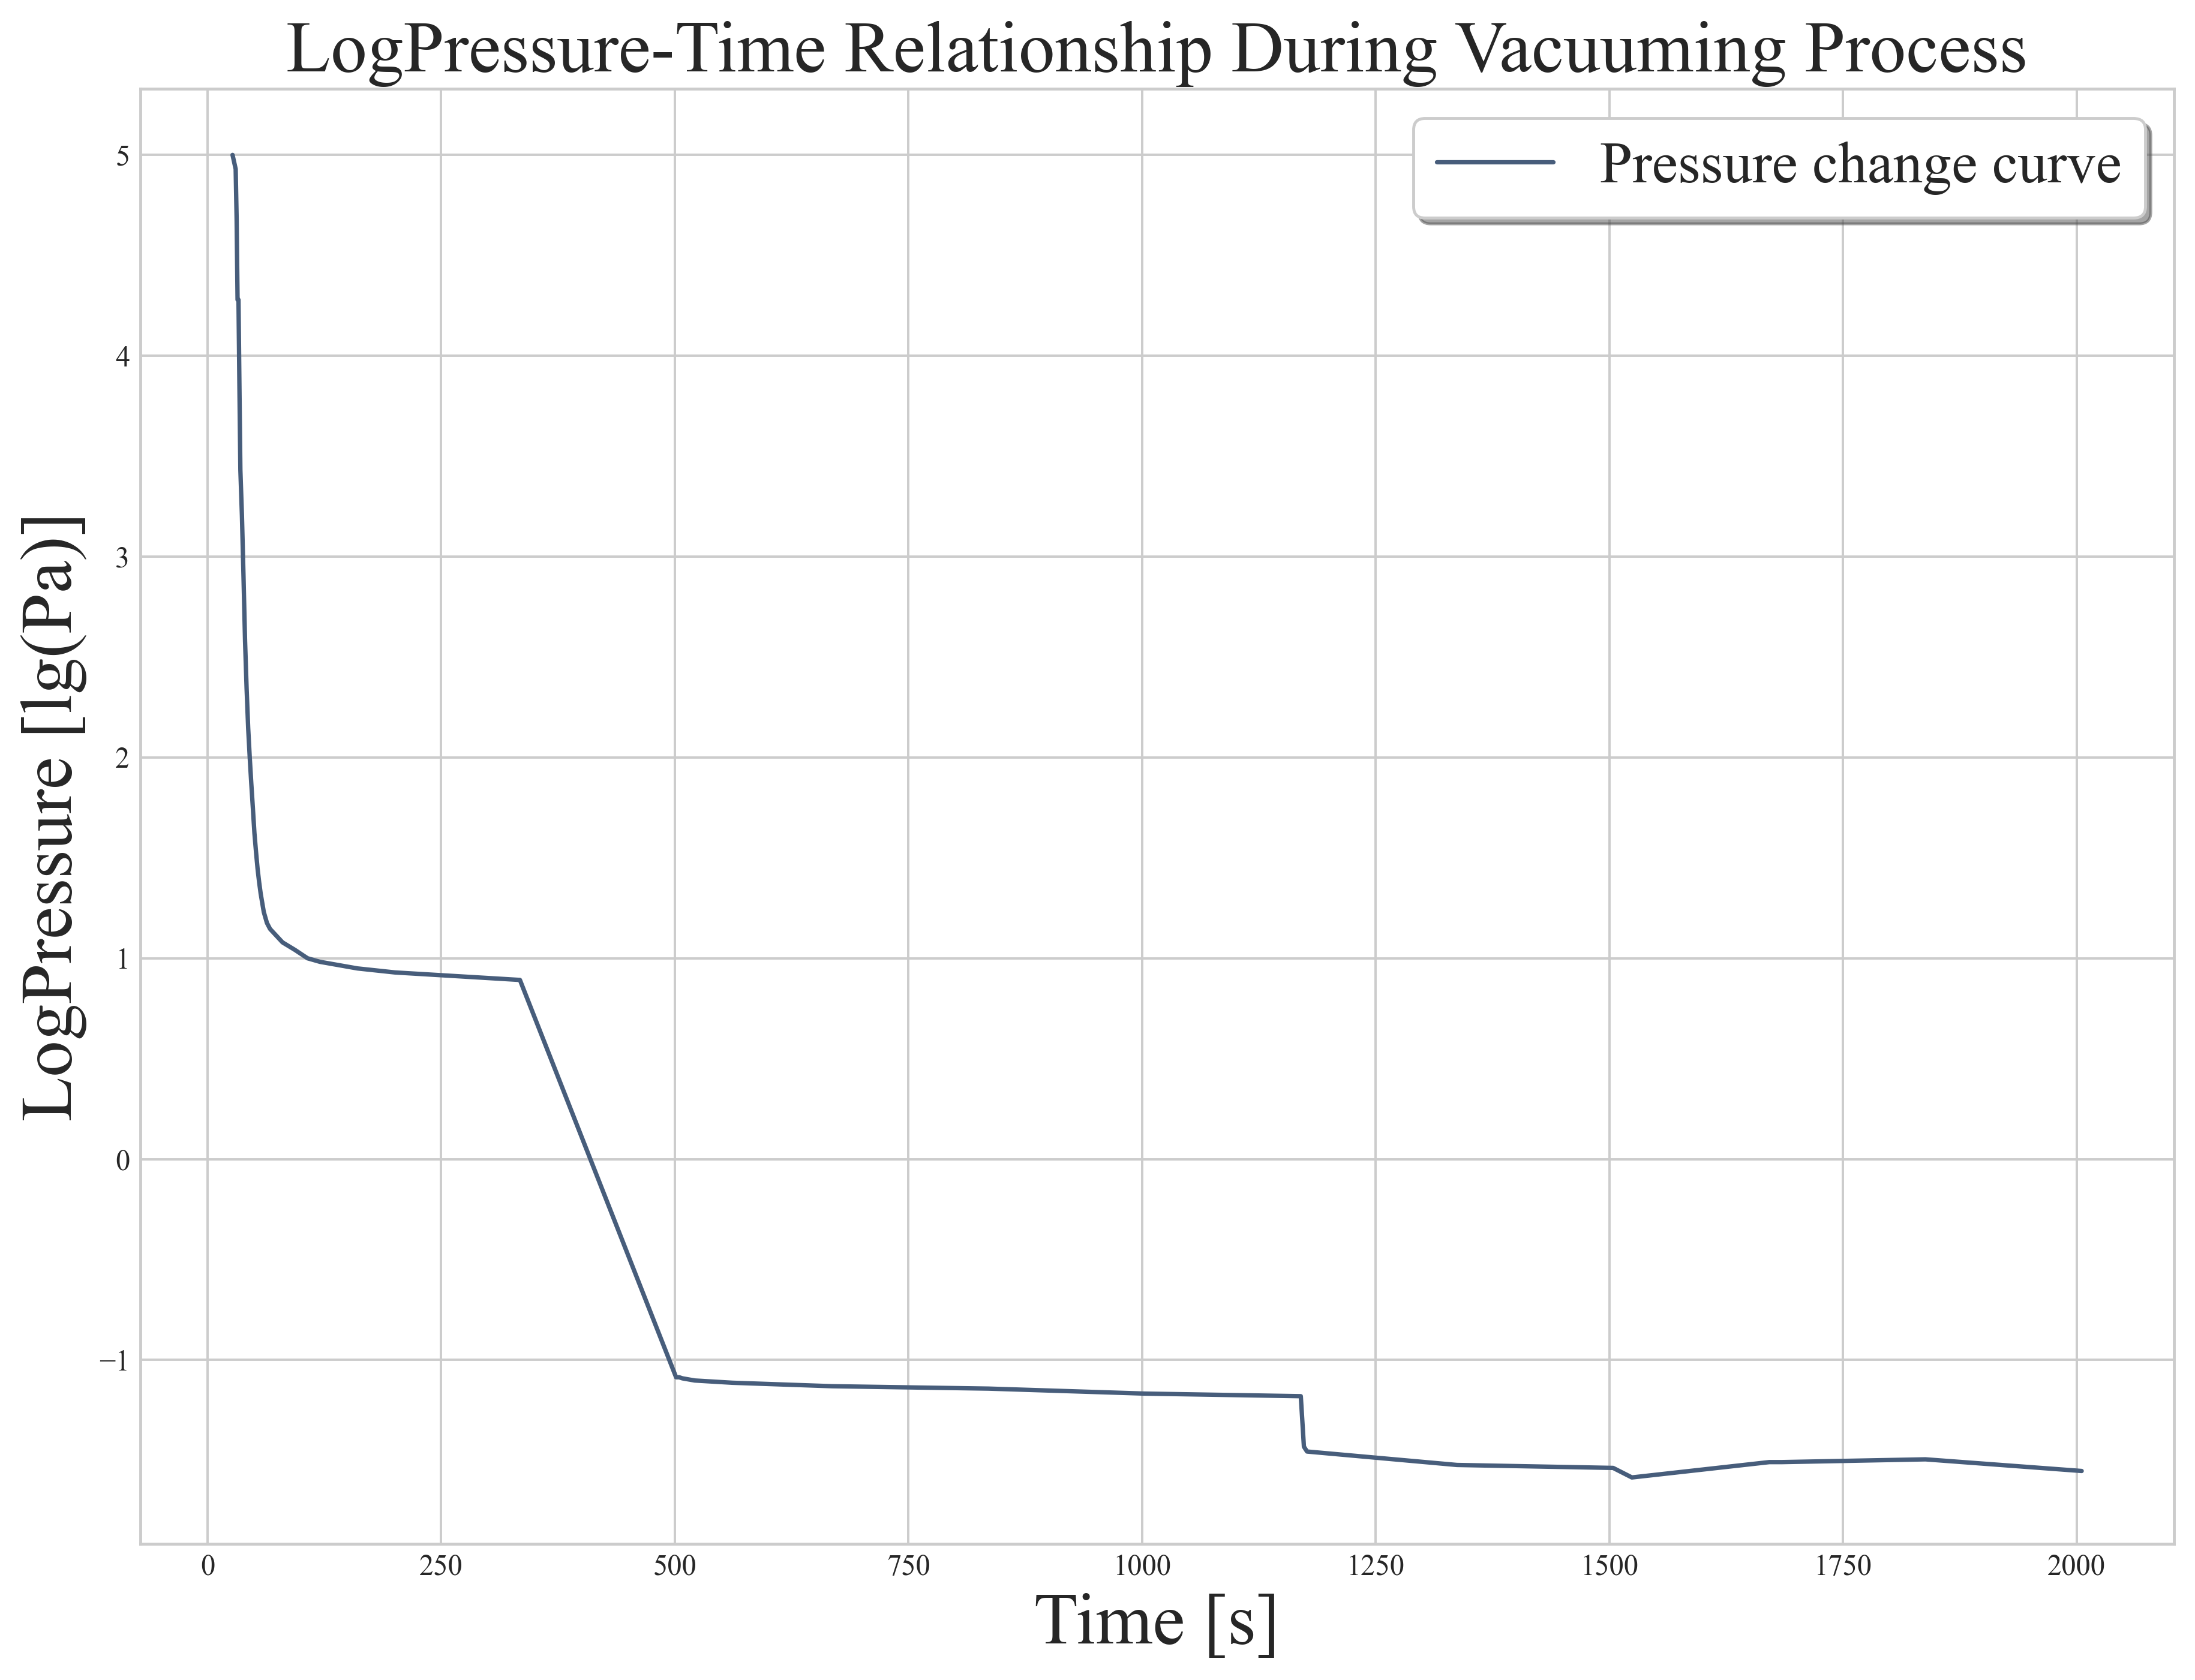
\includegraphics[width=0.7\linewidth]{images/APL1_2_exp1_down}
		\caption{抽真空过程压强-时间关系}
		\label{fig:apl12exp1down}
	\end{figure}
	
	\begin{figure}[htbp]
		\centering
		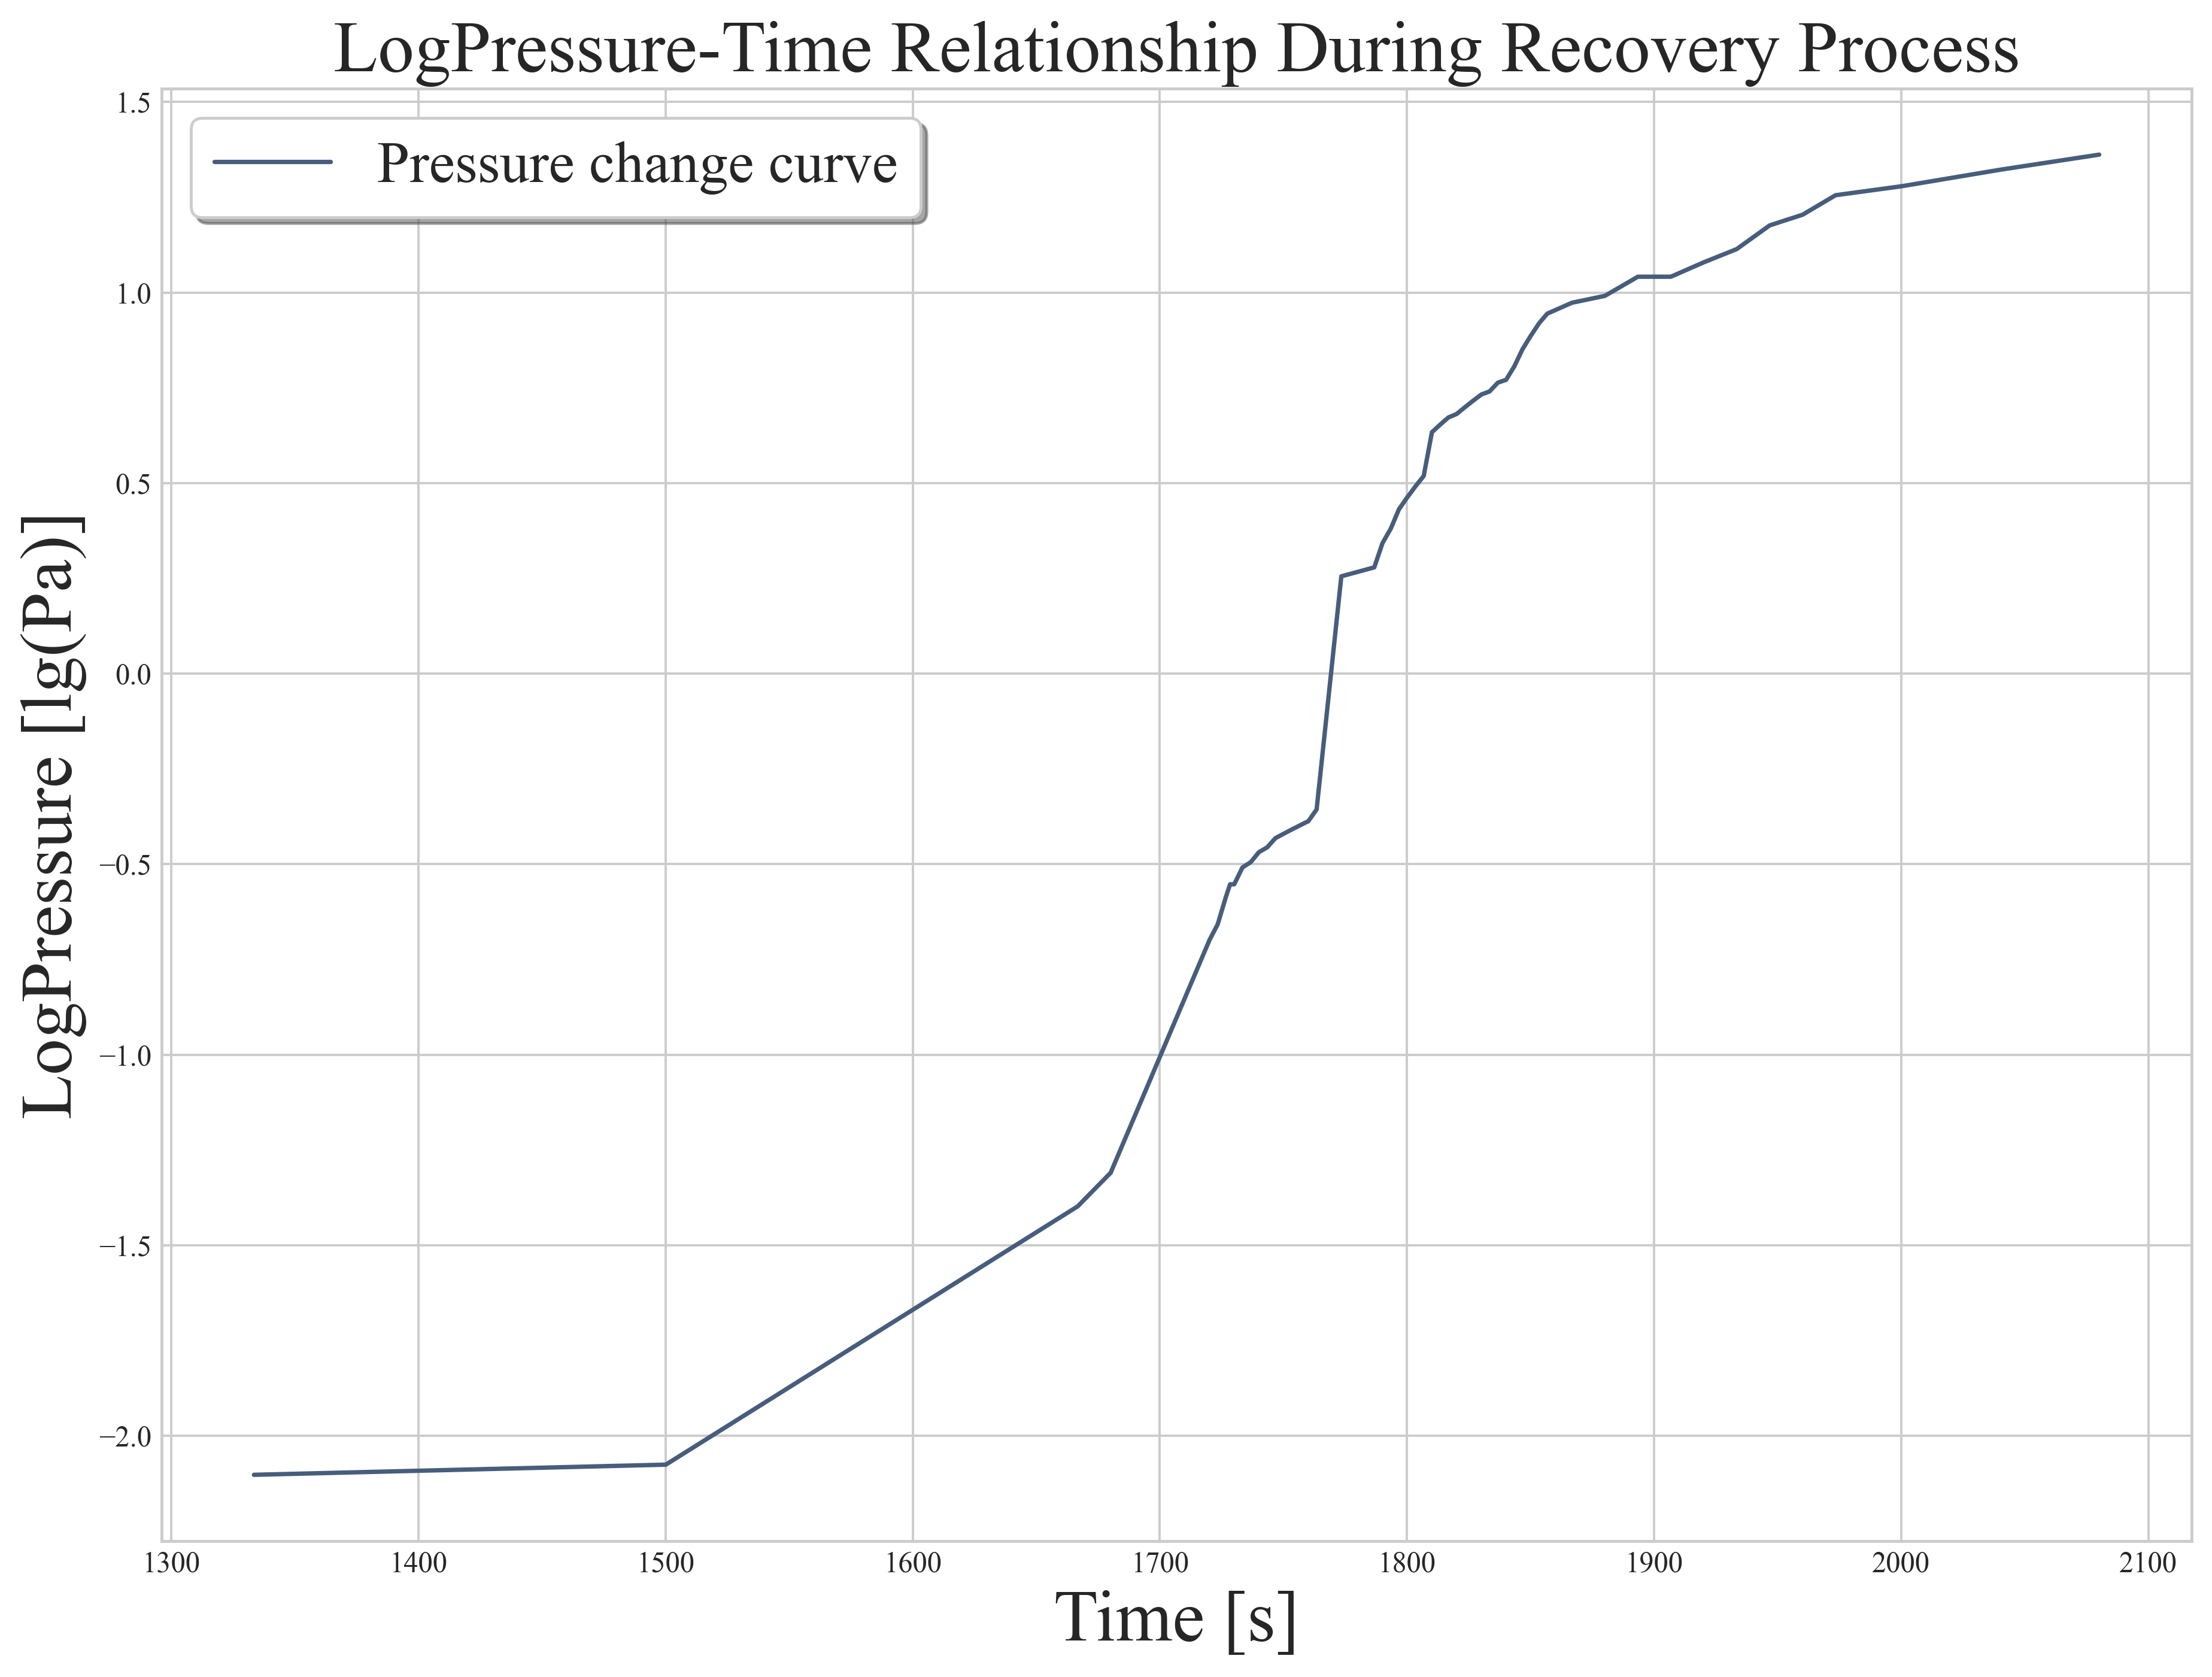
\includegraphics[width=0.7\linewidth]{images/APL1_2_exp1_up}
		\caption{回升过程压强-时间关系}
		\label{fig:apl12exp1up}
	\end{figure}
	
	\item 【实验二】
	
	首先，两电极间距固定，为$d=60mm$。
	
	利用实验测定的数据绘图，如\cref{fig:apl12exp21}所示。可以发现，击穿电压有最低值，且数据分布基本符合$y=\frac{x}{\ln x}$形式。
	
	\begin{figure}[htbp]
		\centering
		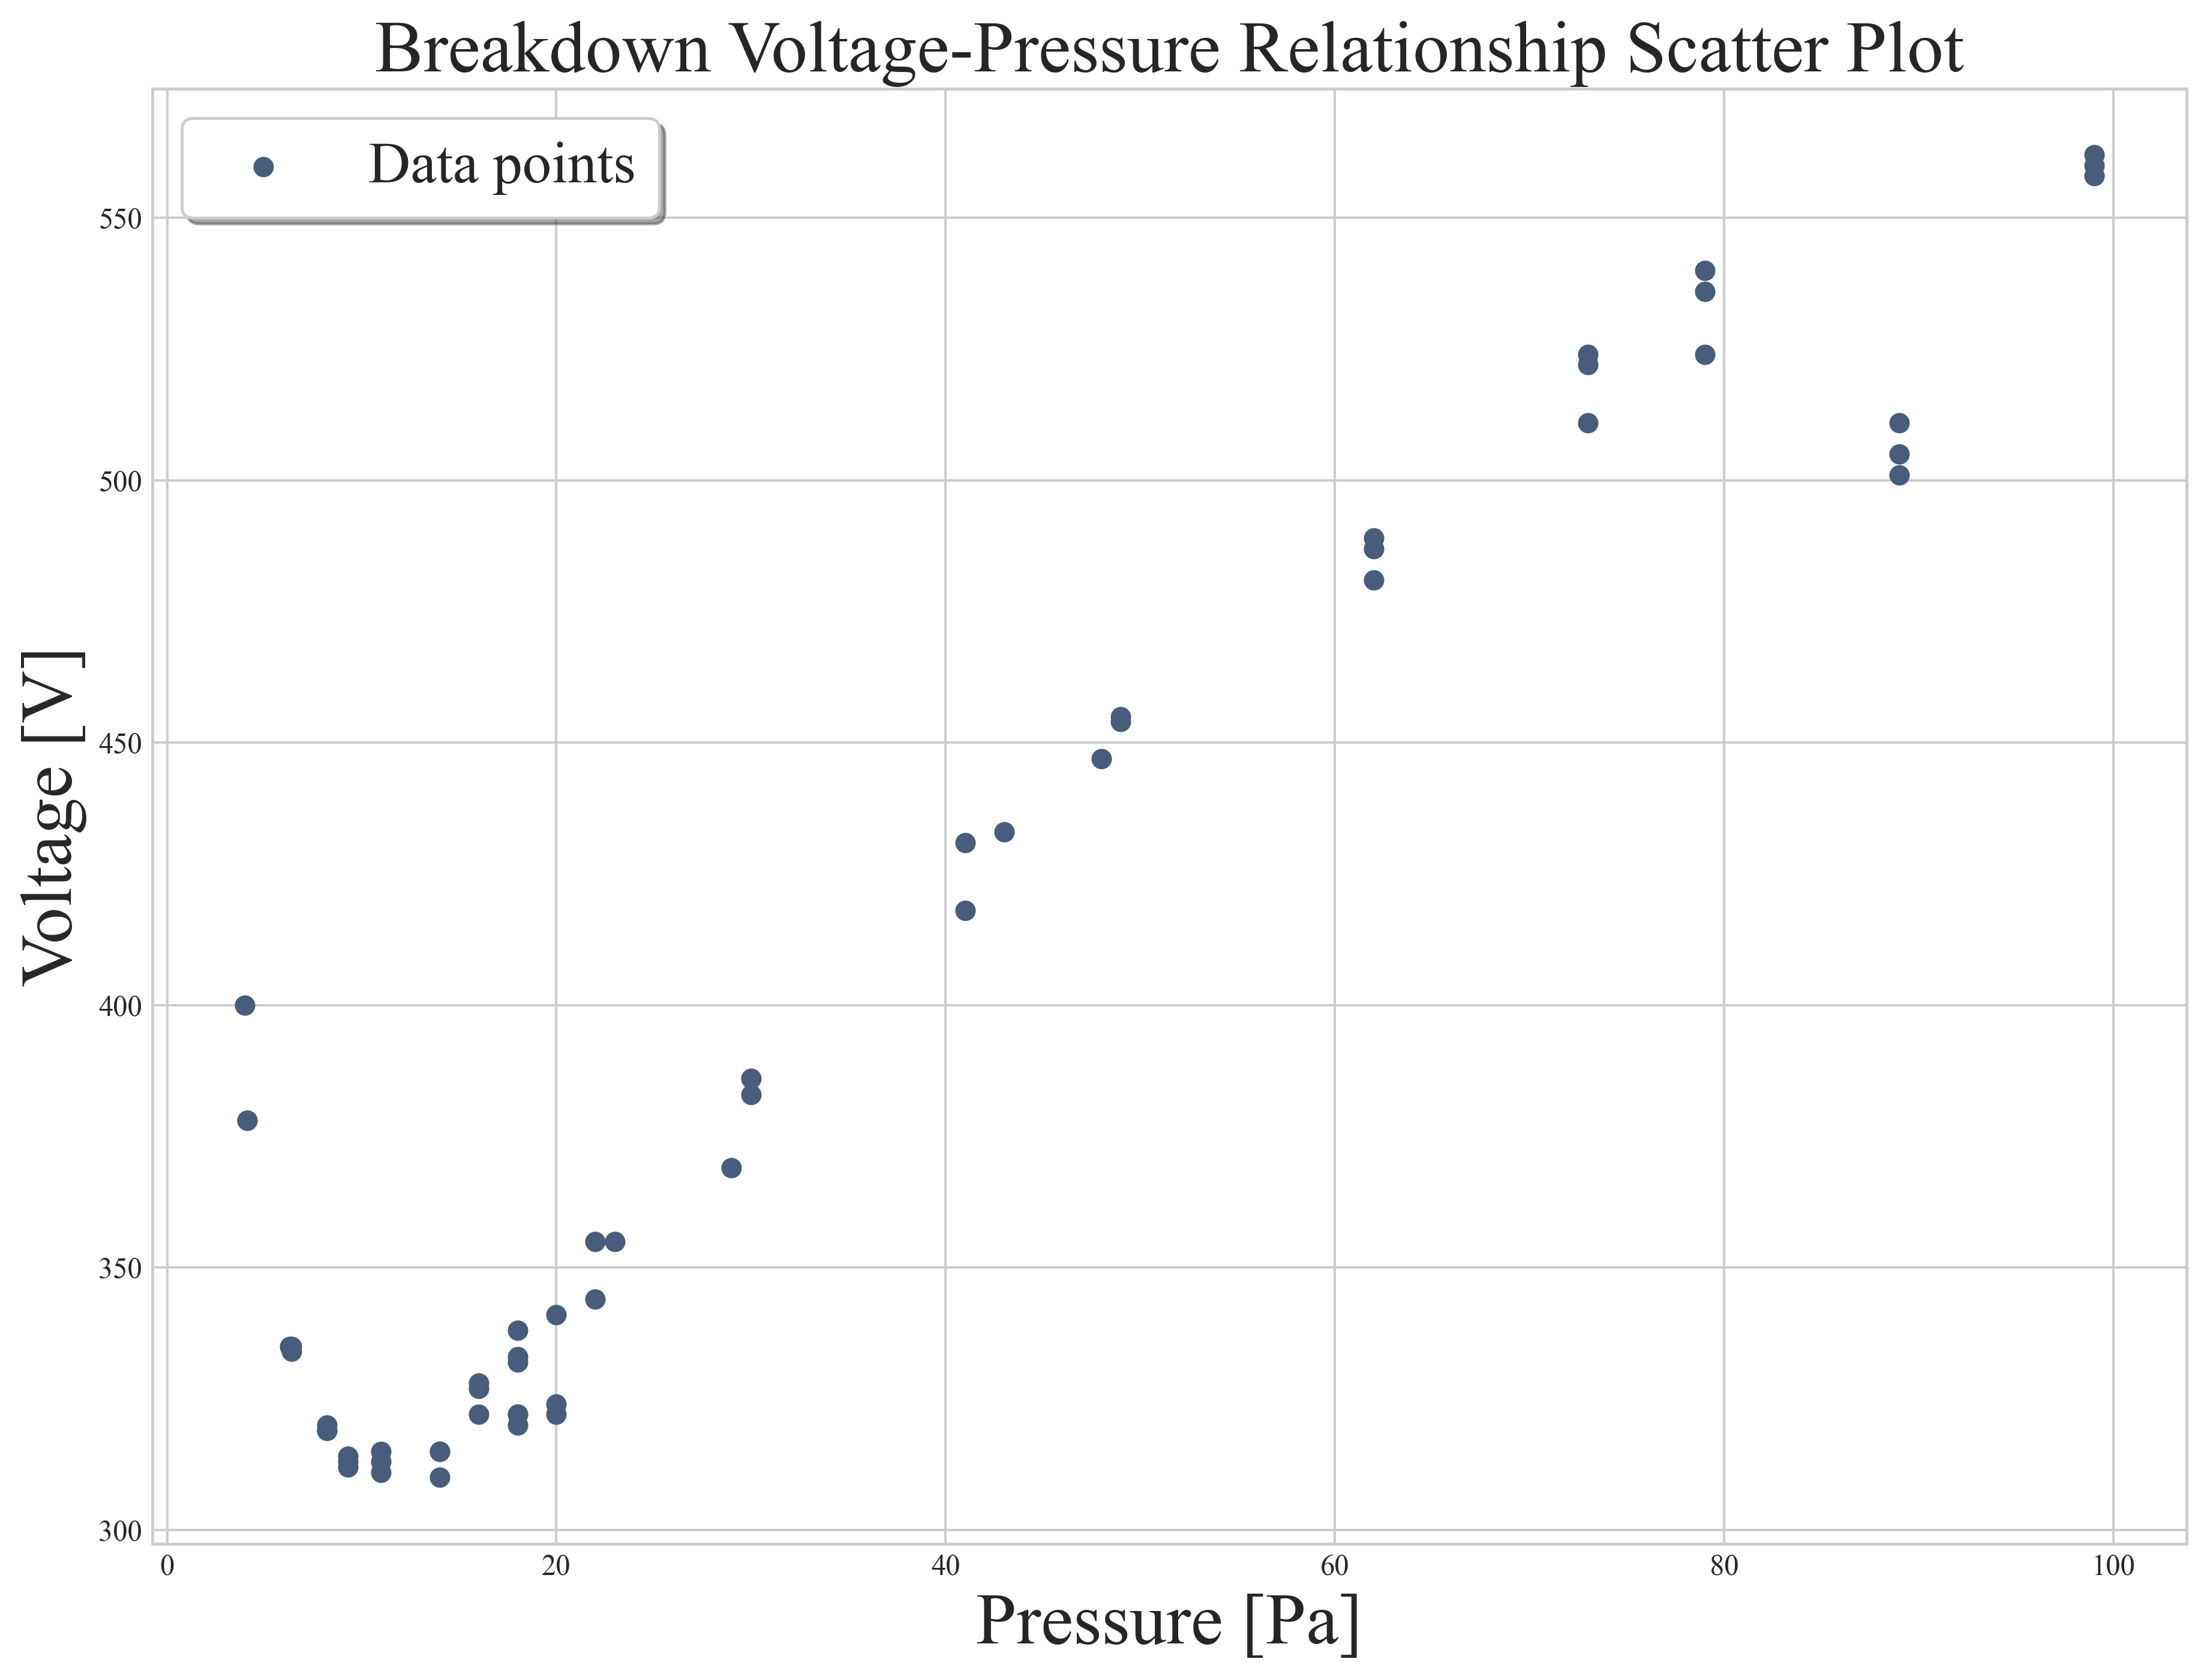
\includegraphics[width=0.7\linewidth]{images/APL1_2_exp2_1}
		\caption{击穿电压-压强关系（实验测定数据点）}
		\label{fig:apl12exp21}
	\end{figure}
	
	\item 【实验三】
	
	通过实验，测定He、Ar和Ne的放电光谱，然后编写脚本寻找了三条主要谱线，结果如\cref{fig:apl12exp3he}、\cref{fig:apl12exp3ar}和\cref{fig:apl12exp3ne}所示。
	
	\begin{figure}
		\centering
		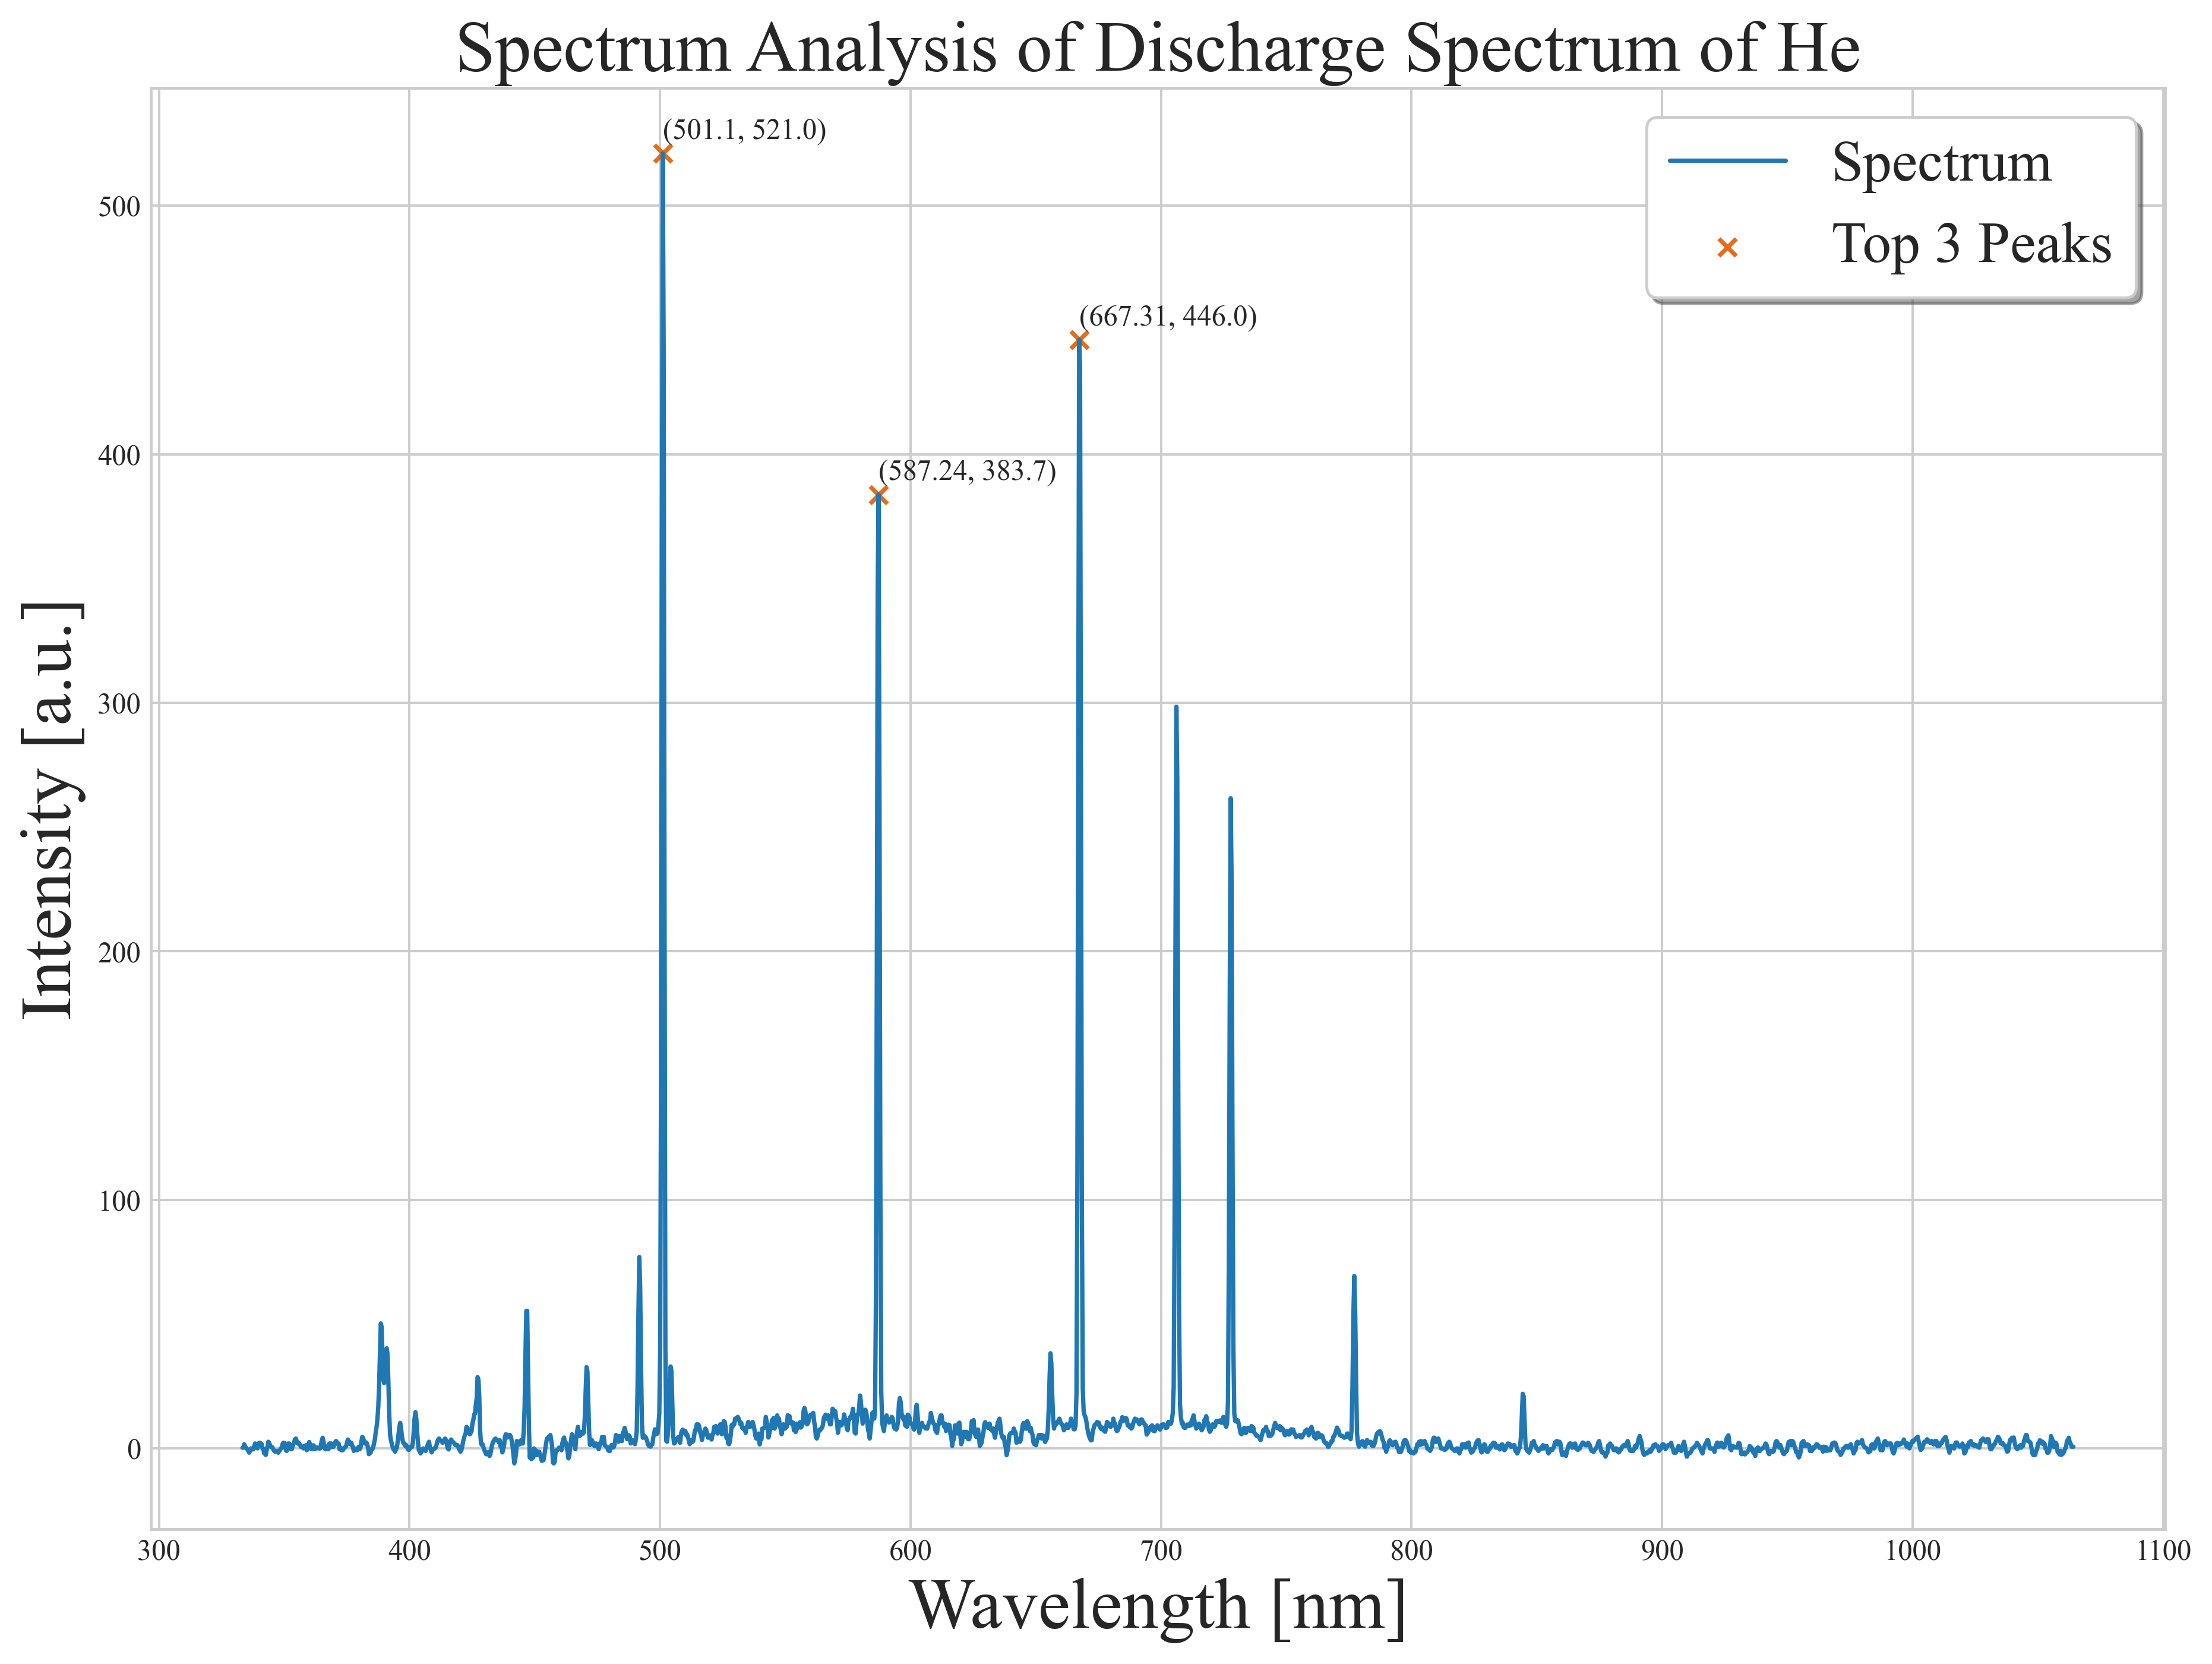
\includegraphics[width=0.7\linewidth]{images/APL1_2_exp3_He}
		\caption{He放电谱线}
		\label{fig:apl12exp3he}
	\end{figure}
	
	\begin{figure}
		\centering
		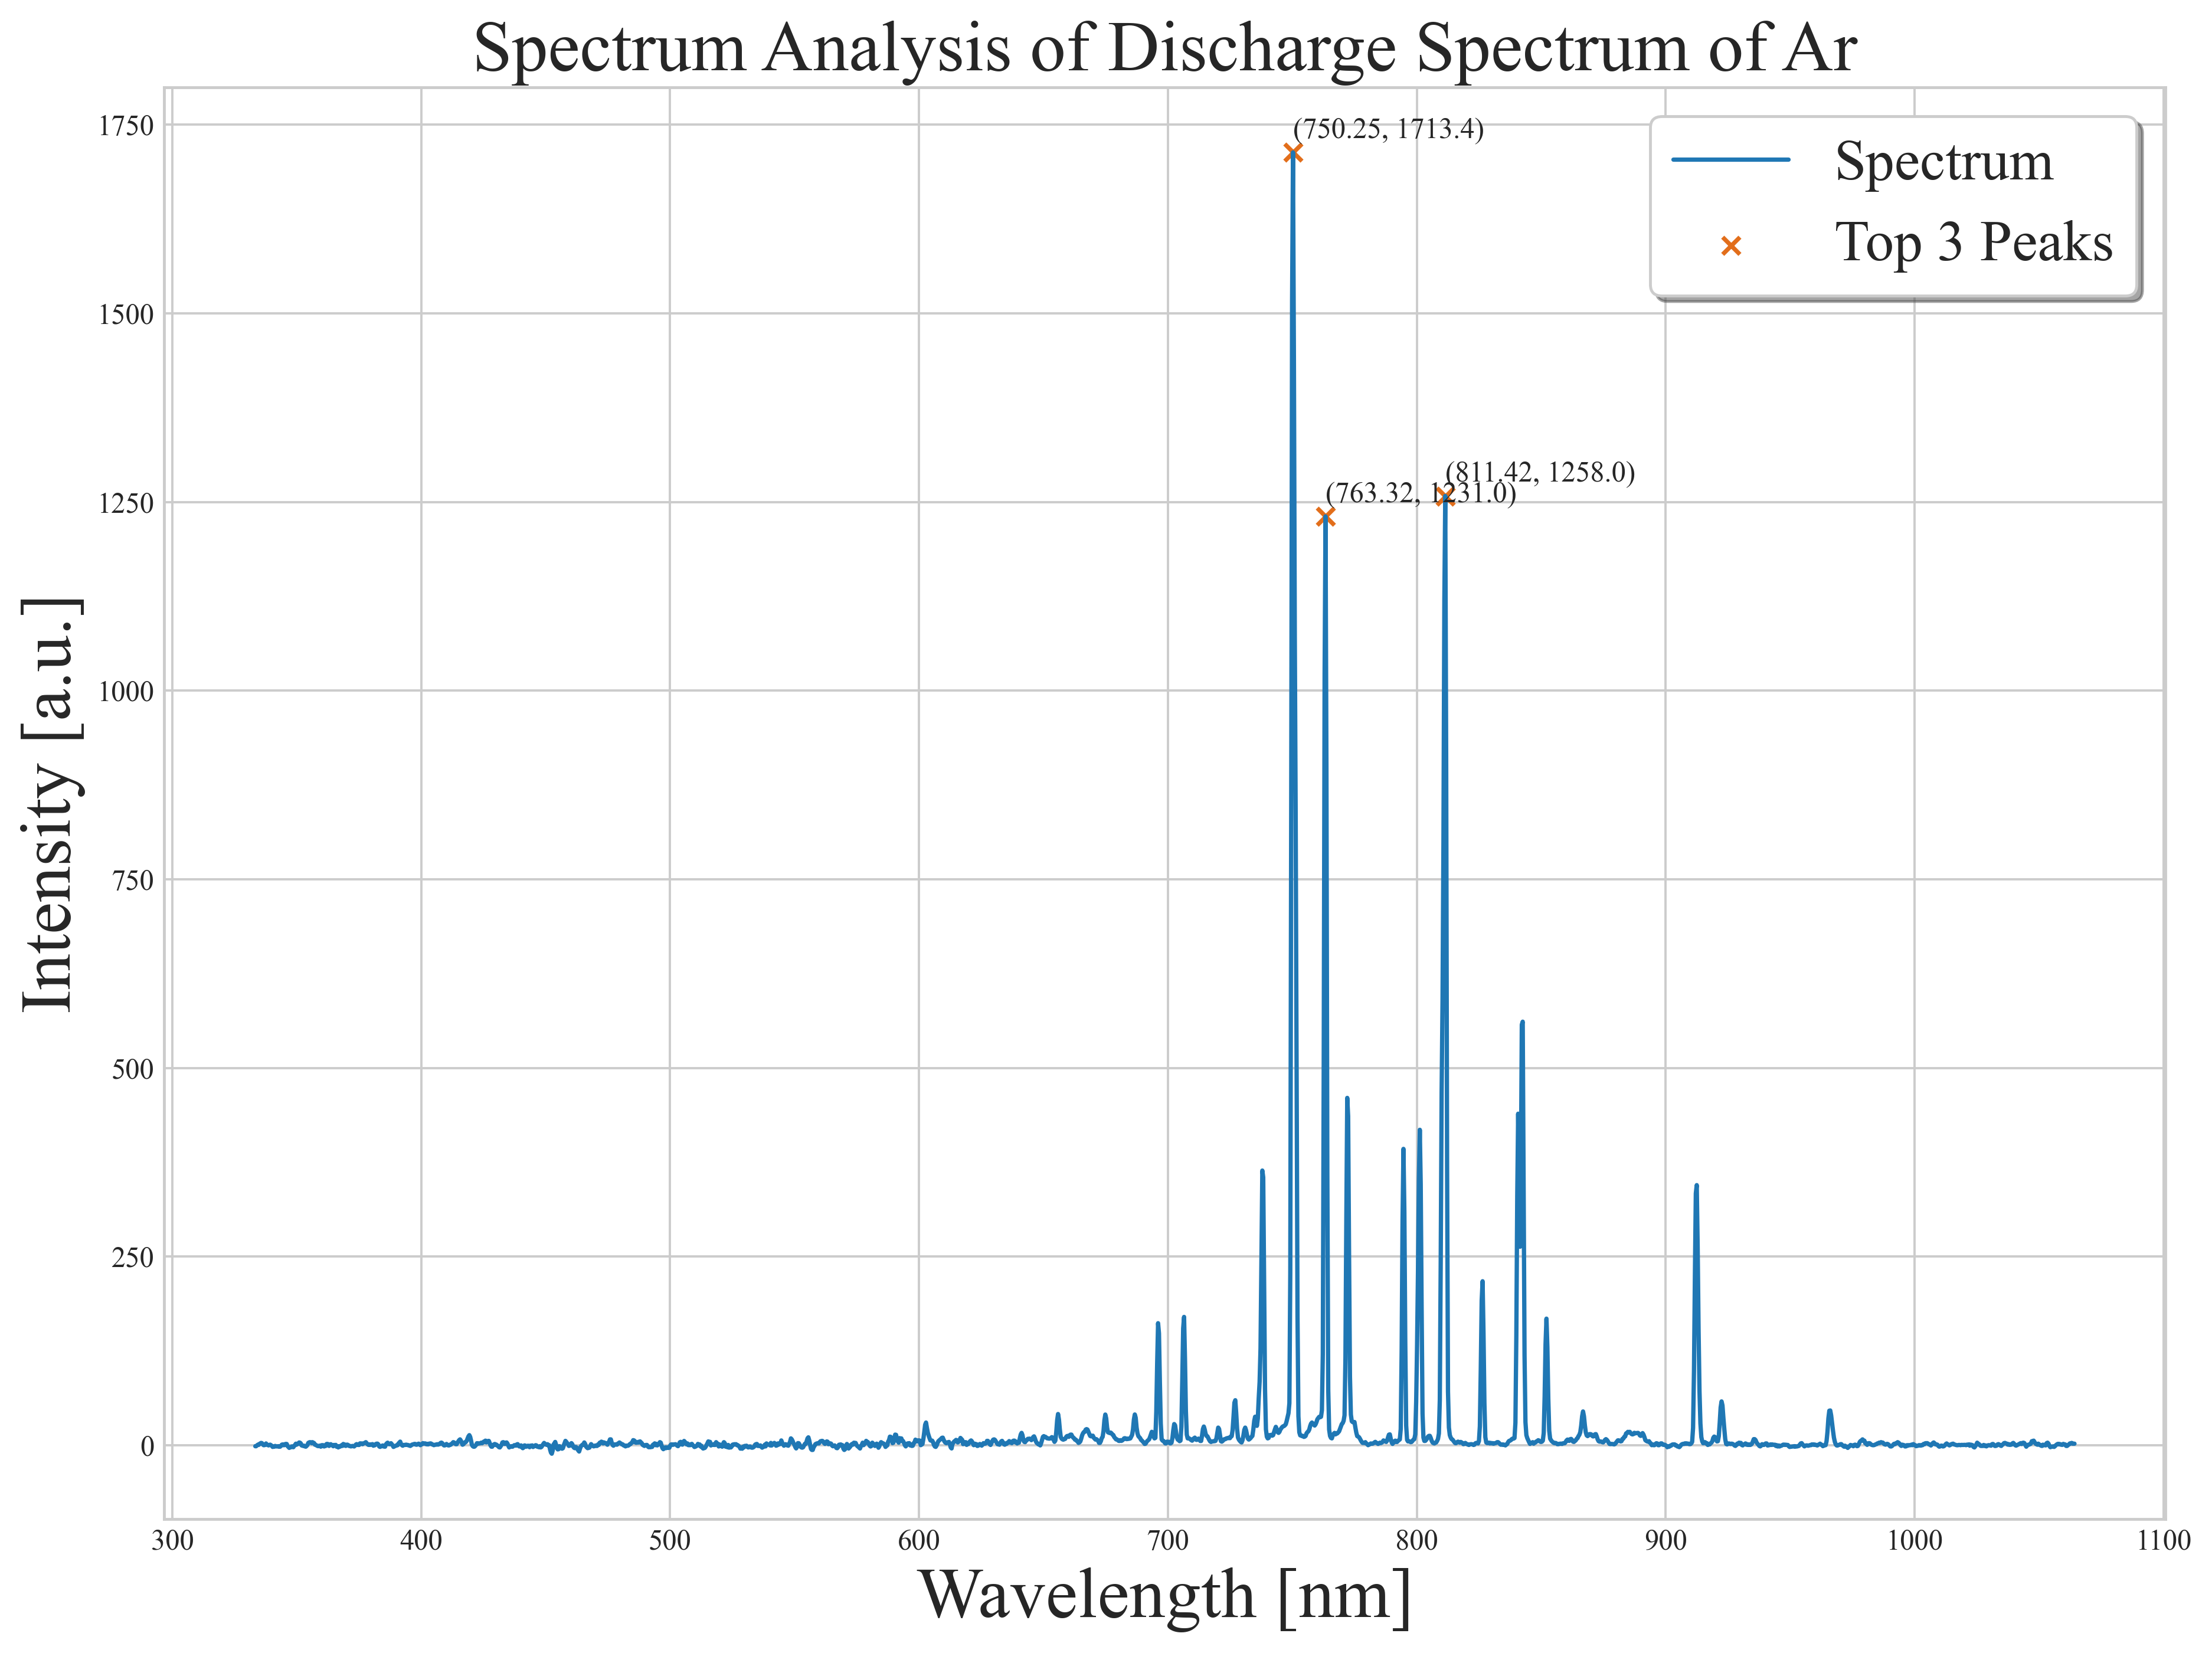
\includegraphics[width=0.7\linewidth]{images/APL1_2_exp3_Ar}
		\caption{Ar放电谱线}
		\label{fig:apl12exp3ar}
	\end{figure}
	
	\begin{figure}
		\centering
		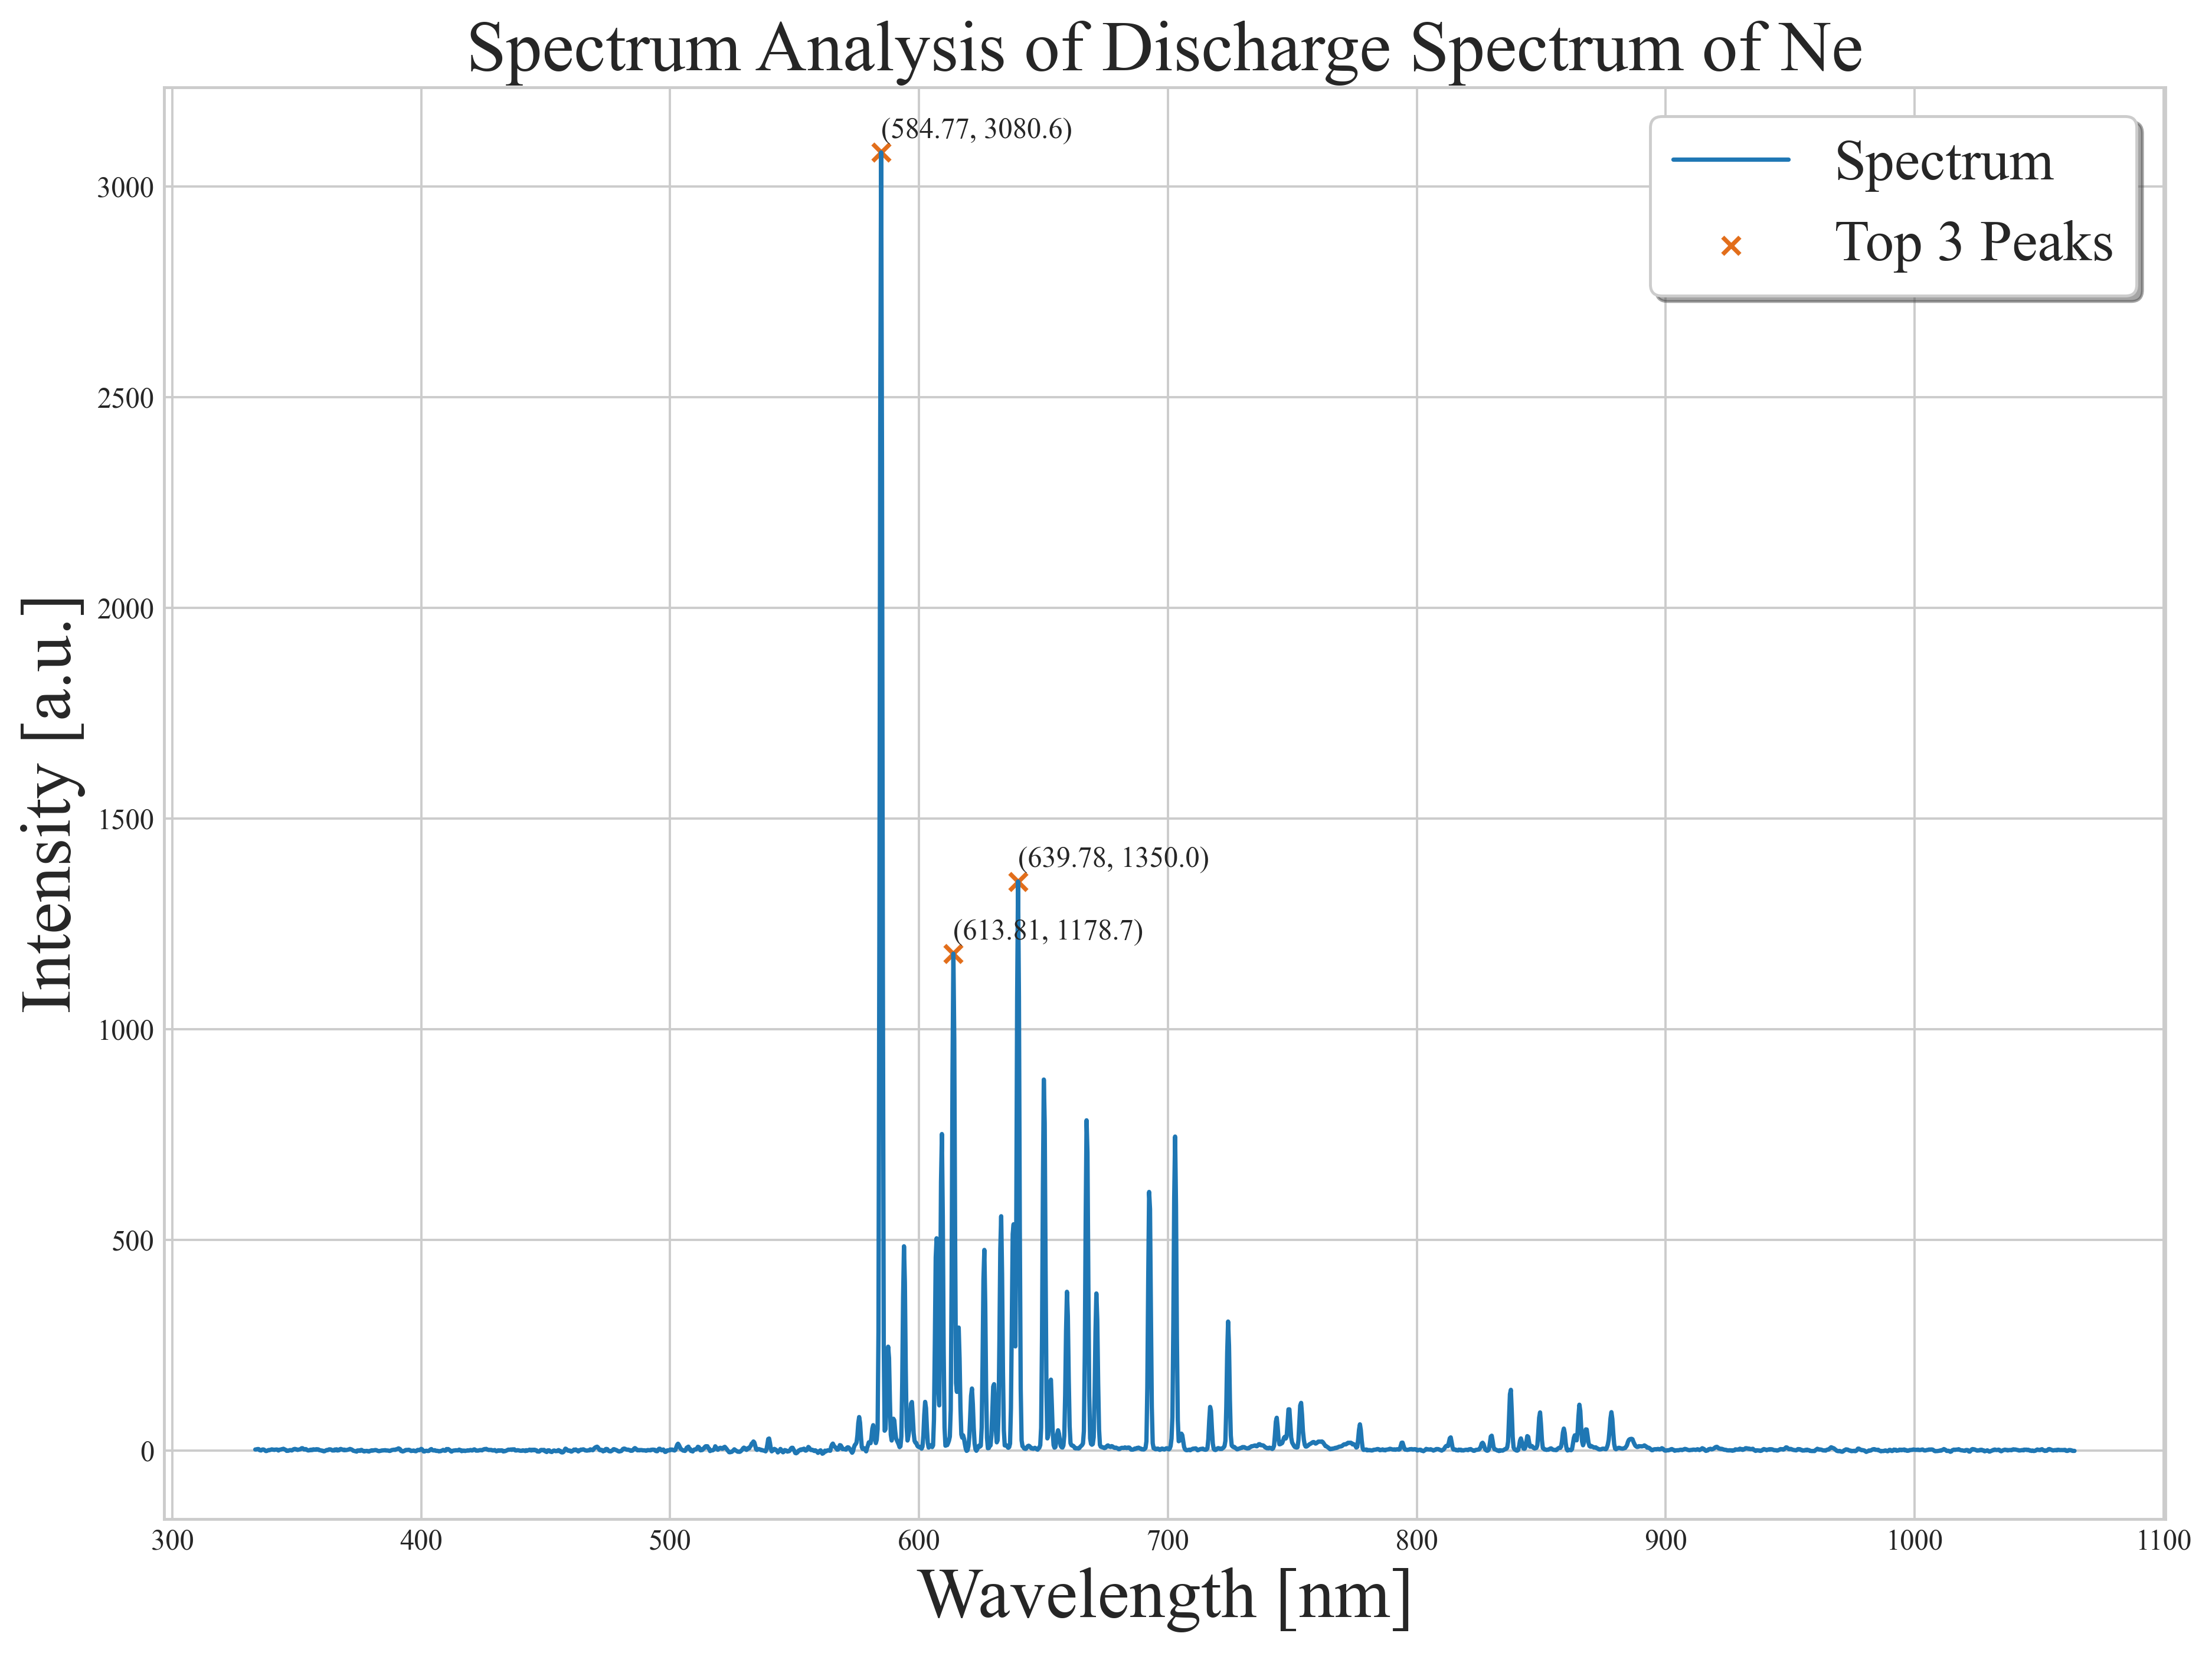
\includegraphics[width=0.7\linewidth]{images/APL1_2_exp3_Ne}
		\caption{Ne放电谱线}
		\label{fig:apl12exp3ne}
	\end{figure}
	
	\item 【实验四】
	
	\begin{figure}[htbp]
		\centering
		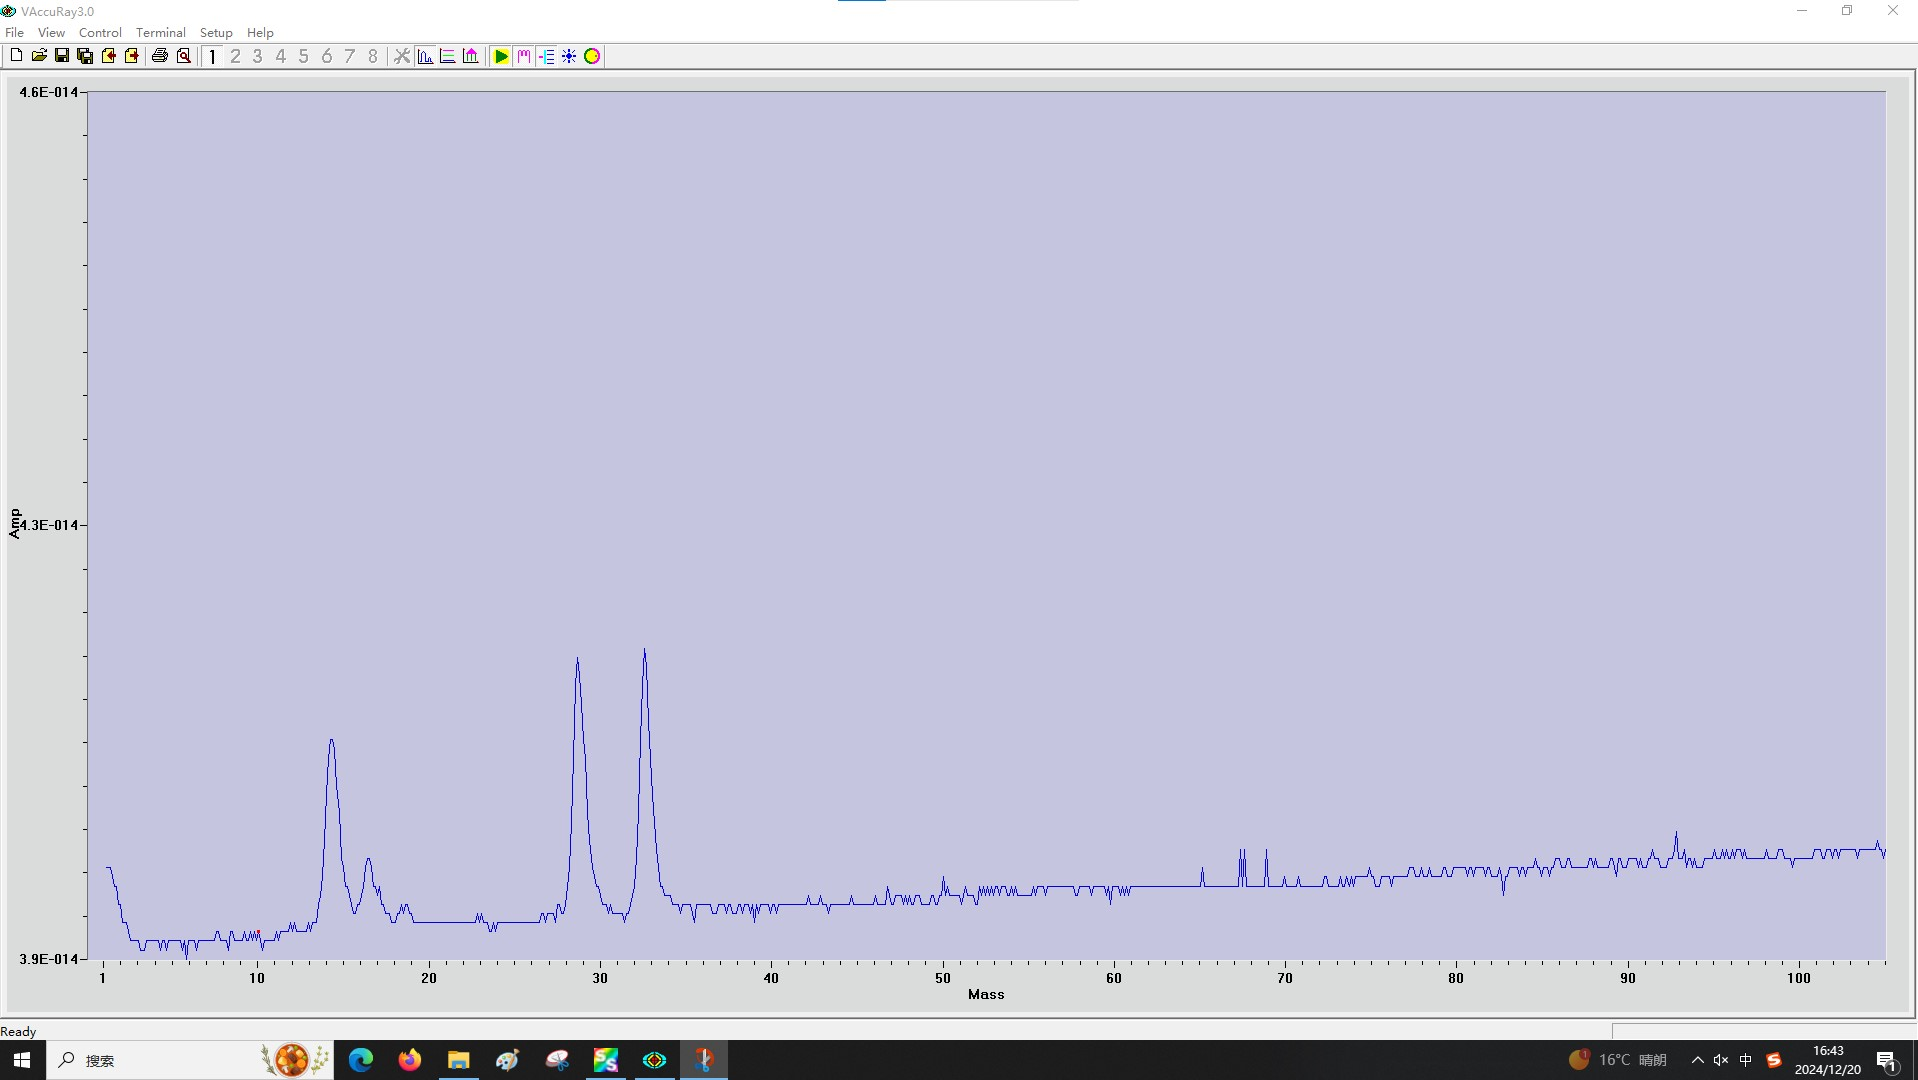
\includegraphics[width=0.7\linewidth]{images/APL1_2_4_air_O}
		\caption{空气的质谱仪谱线（实验测定）}
		\label{fig:apl124airo}
	\end{figure}
	
	\begin{figure}[htbp]
		\centering
		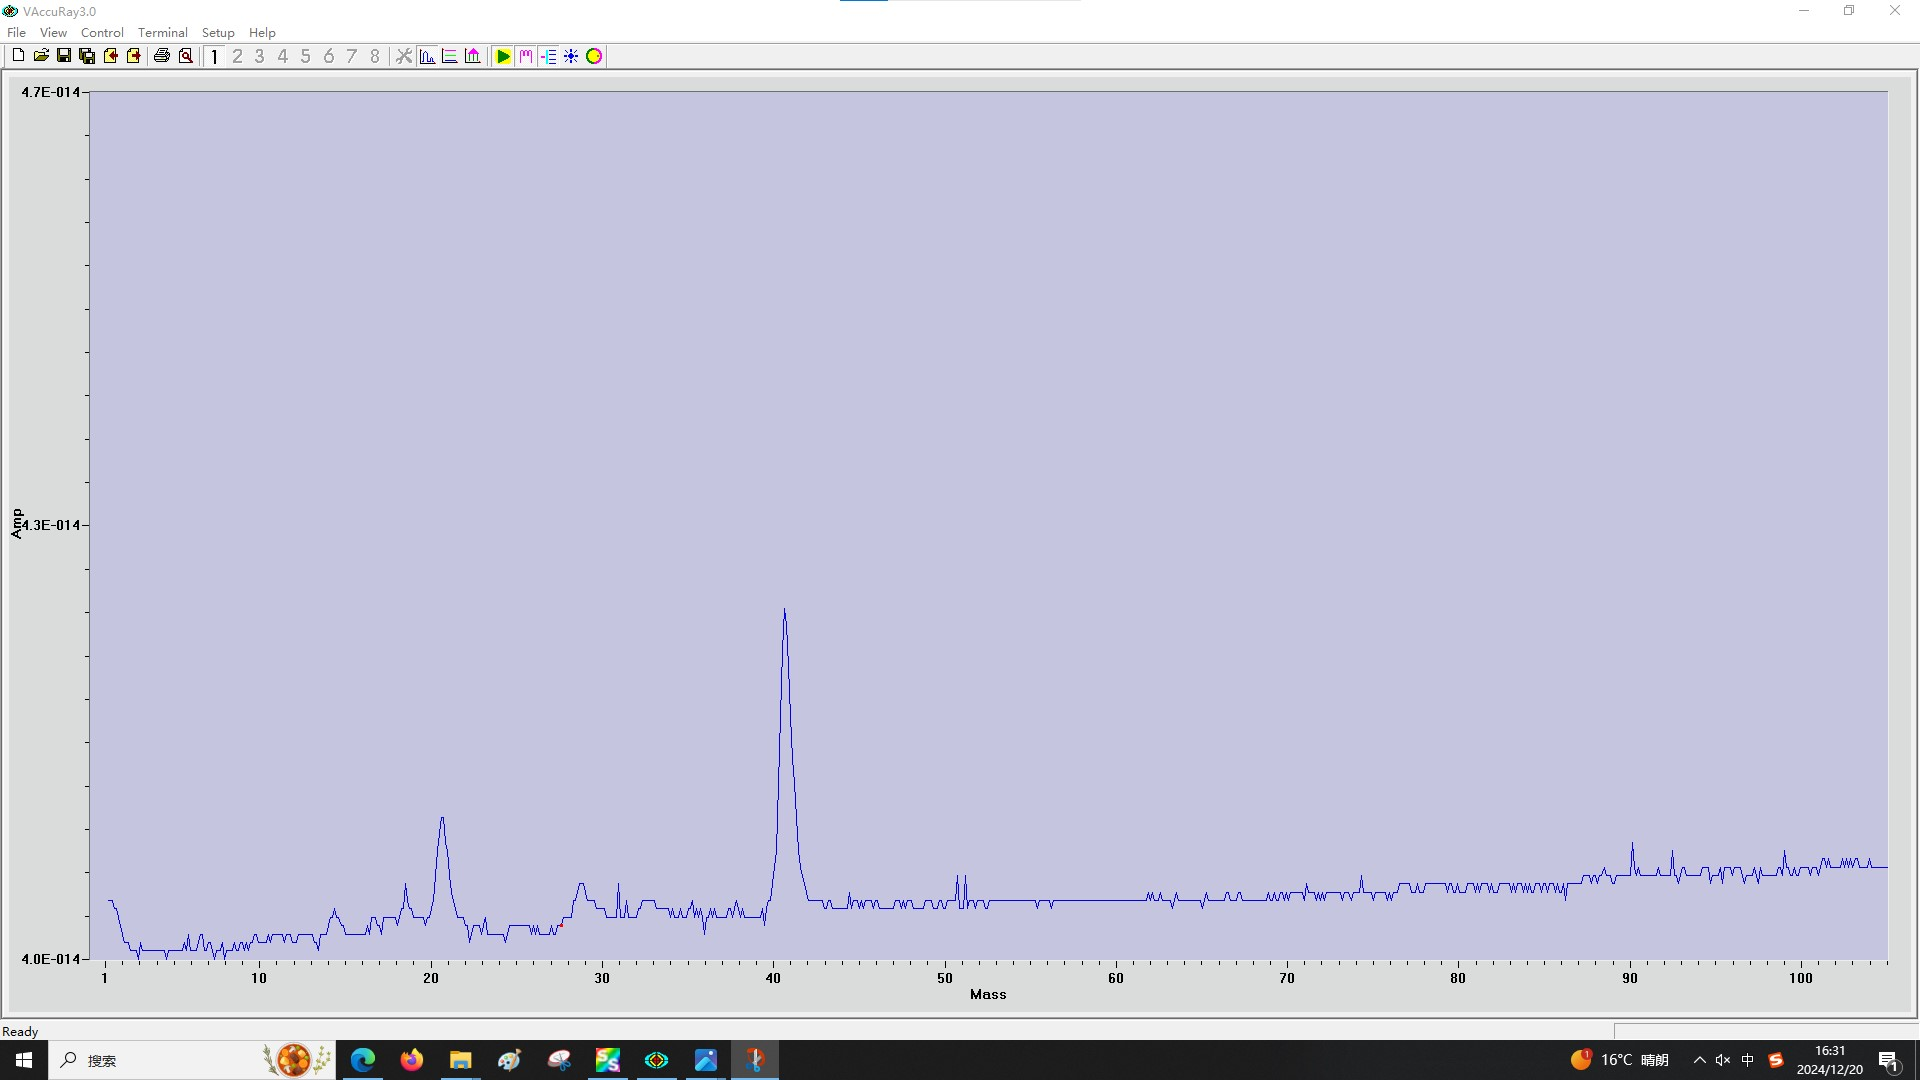
\includegraphics[width=0.7\linewidth]{images/APL1_2_4_Ar_O}
		\caption{Ar的质谱仪谱线（实验测定）}
		\label{fig:apl124aro}
	\end{figure}
	
	\begin{figure}[htbp]
		\centering
		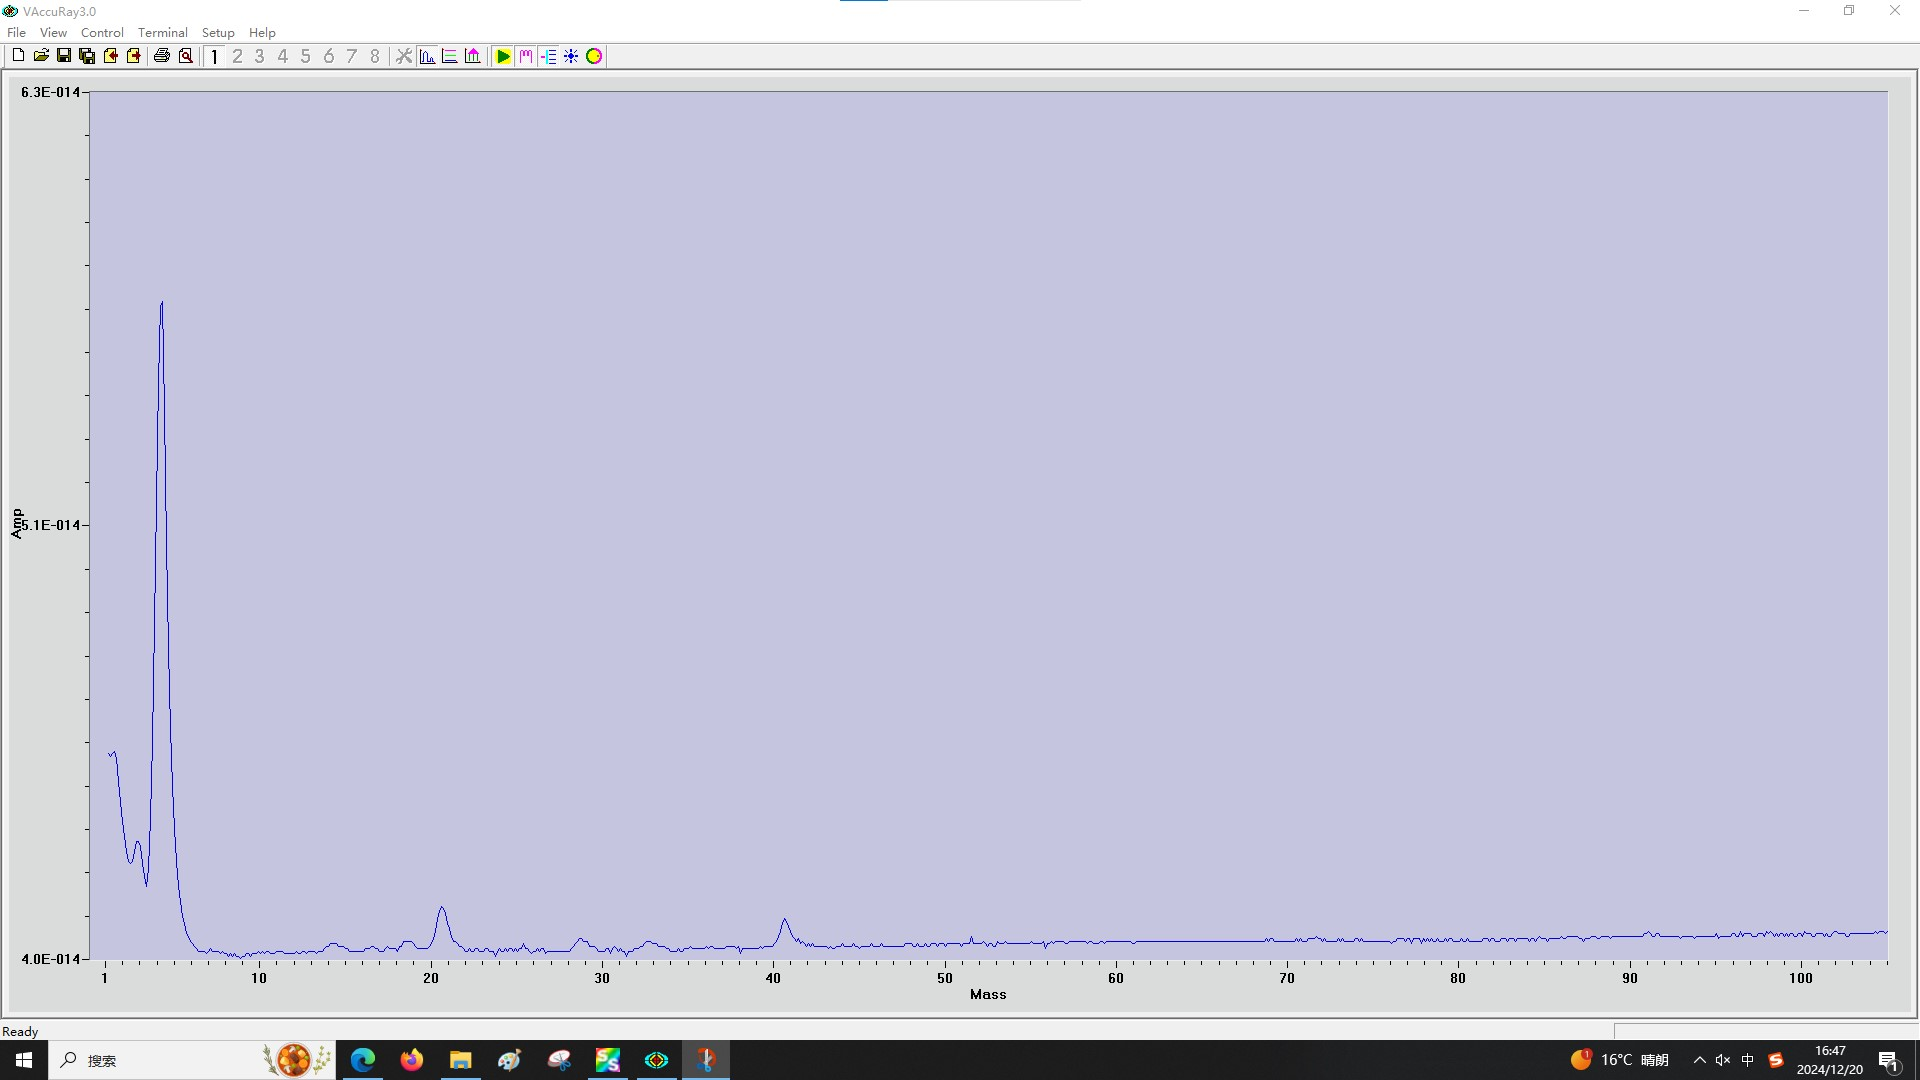
\includegraphics[width=0.7\linewidth]{images/APL1_2_4_He_O}
		\caption{He的质谱仪谱线（实验测定）}
		\label{fig:apl124heo}
	\end{figure}
	
	\begin{figure}[htbp]
		\centering
		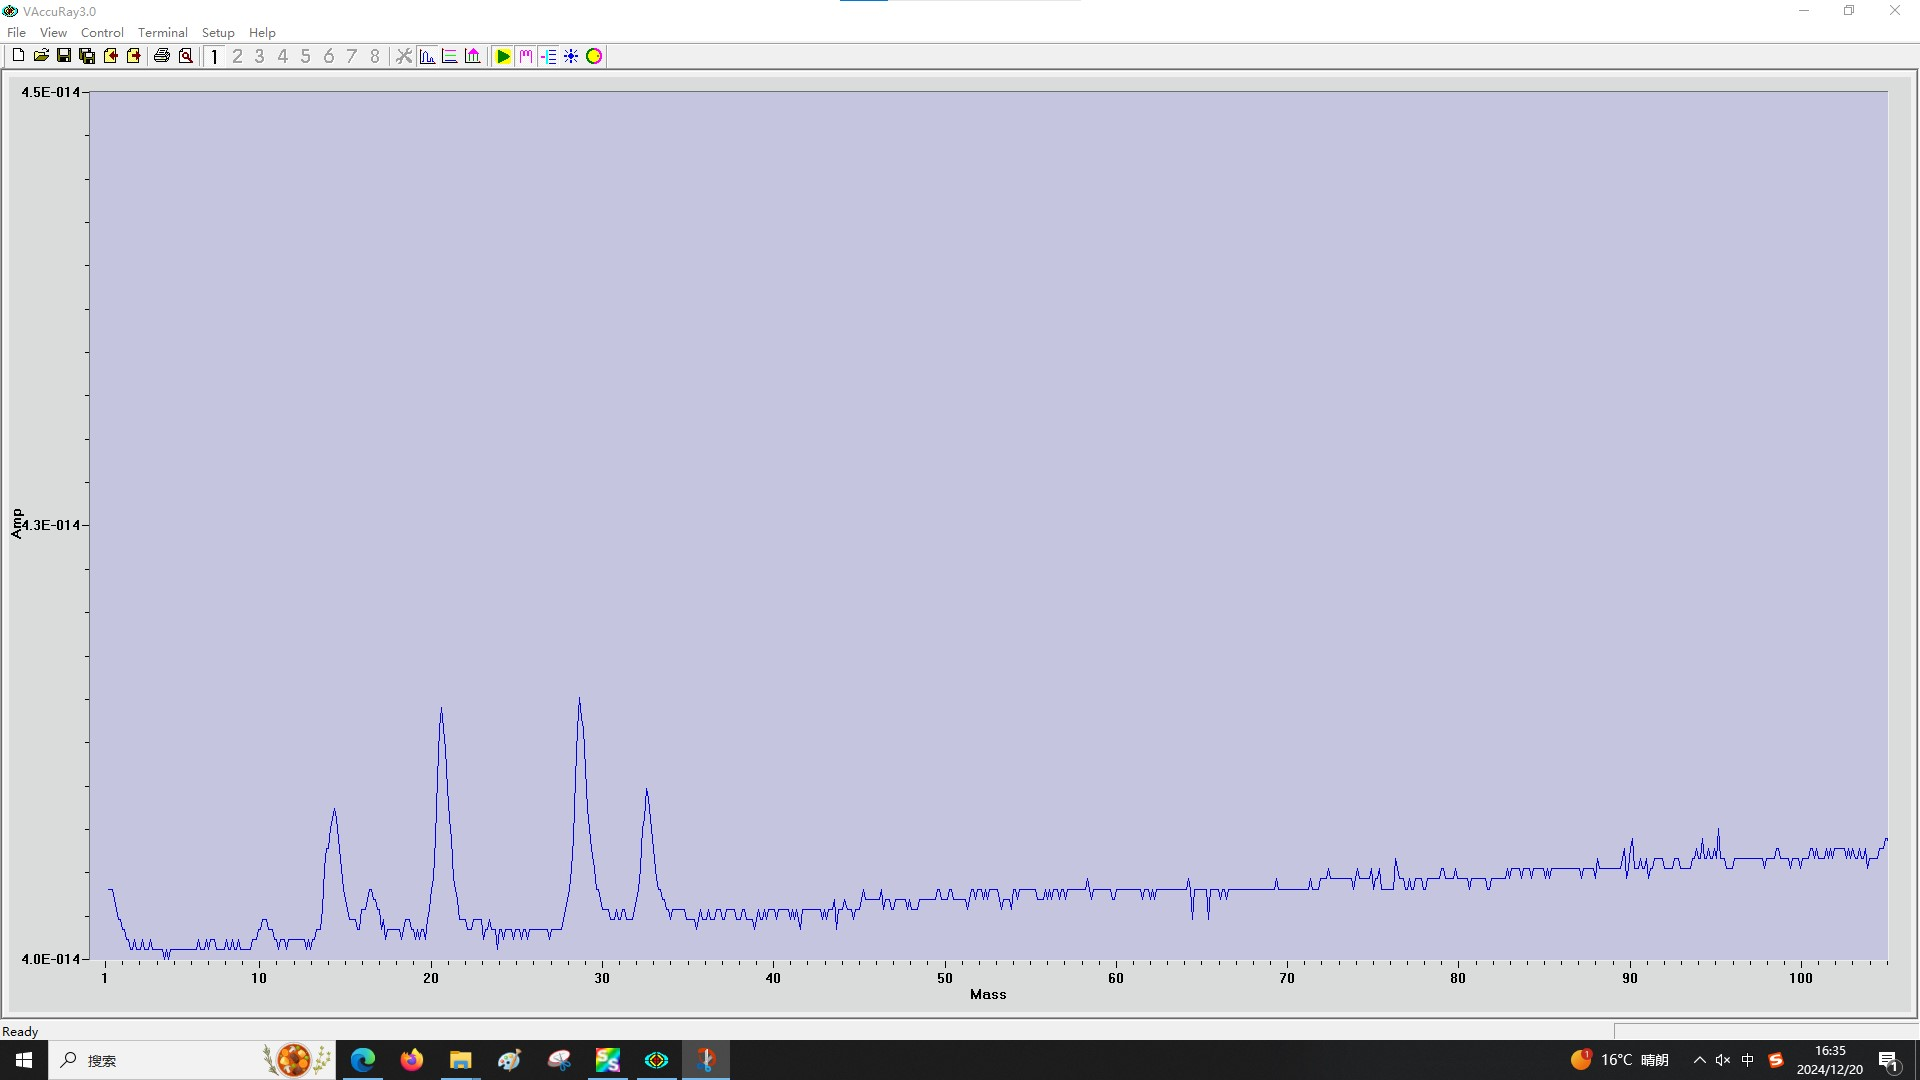
\includegraphics[width=0.7\linewidth]{images/APL1_2_4_Ne_O}
		\caption{Ne的质谱仪谱线}
		\label{fig:apl124neo}
	\end{figure}
	
\end{enumerate}

\textbf{对上述实验结果和数据的分析与讨论详见数据分析部分。}


%---------------------------------------------------------------------
% 原始数据
\subsection{Original Data}
%The original data in the experimental notebook is shown in %\cref{} (signed).

\begin{figure}
	\centering
	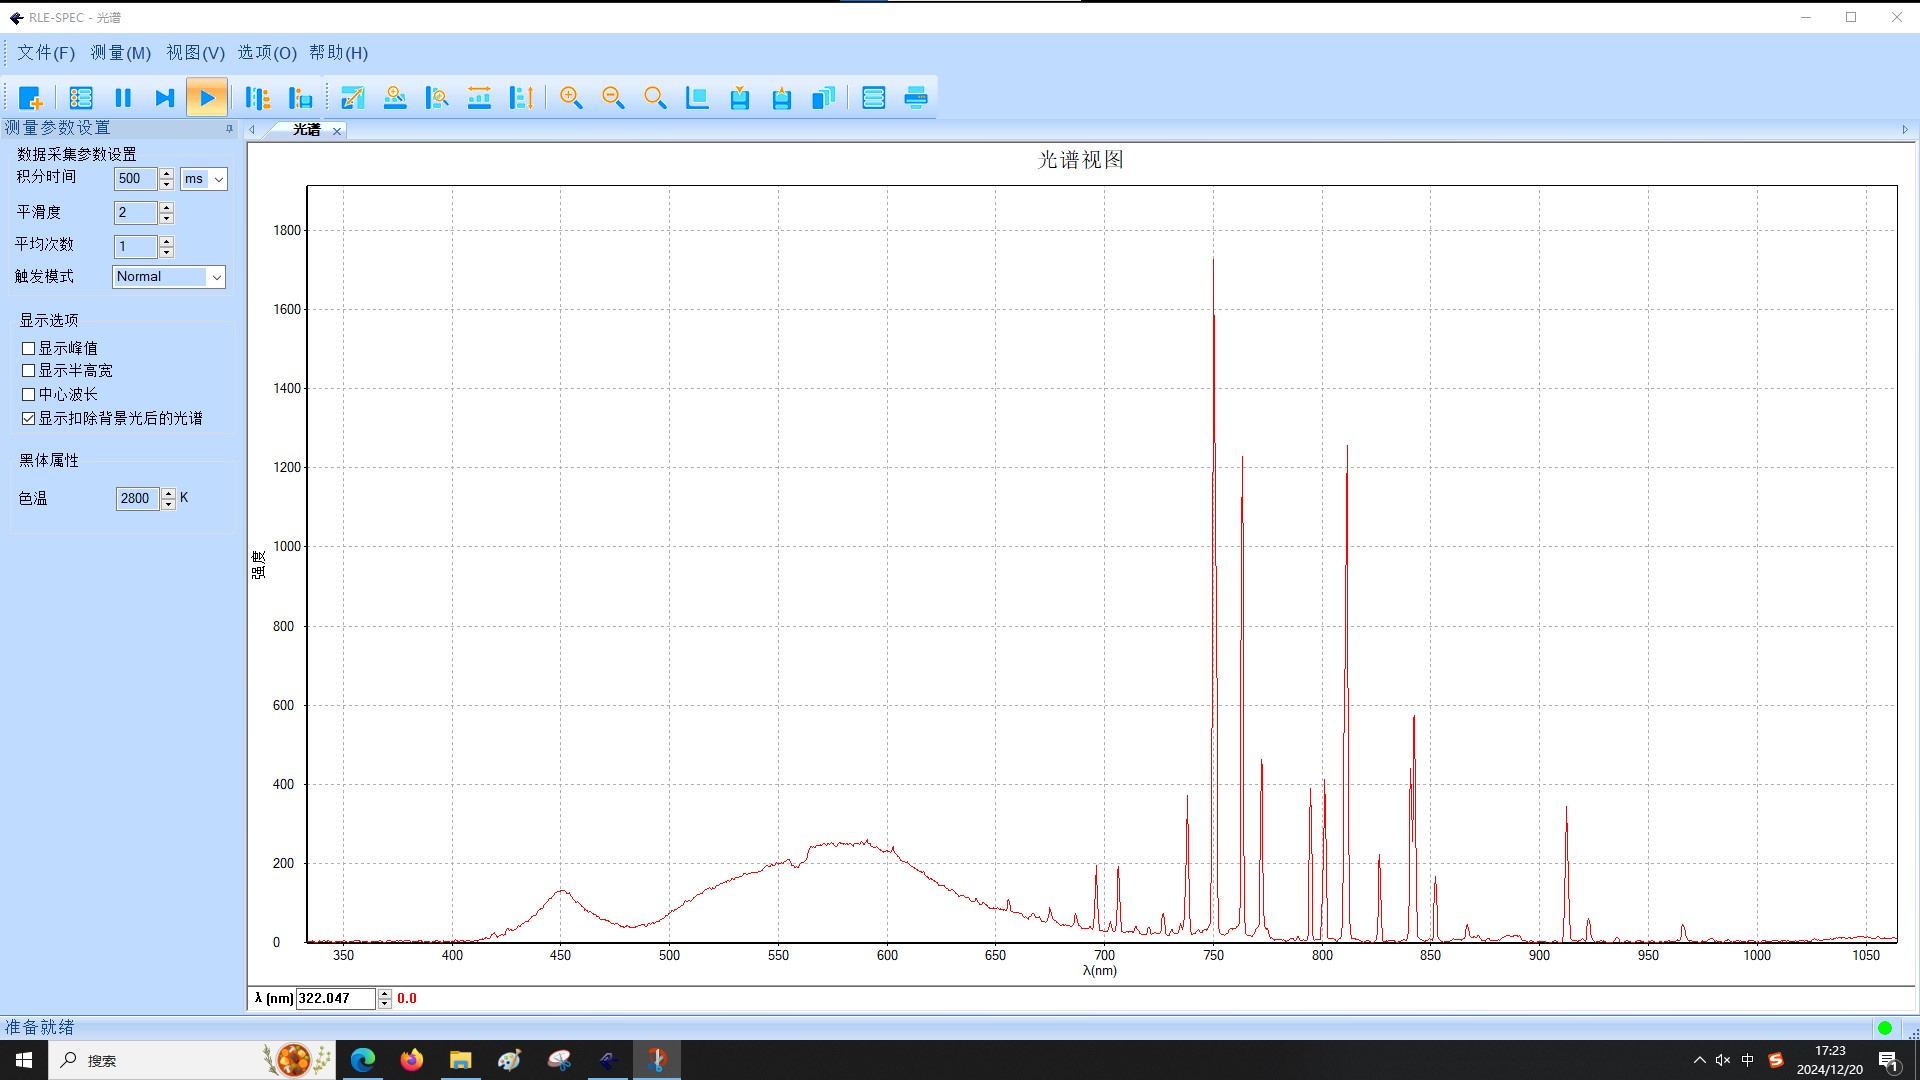
\includegraphics[width=0.6\linewidth]{images/APL1_2_exp3_Ar_O}
	\caption{原始数据展示}
	\label{fig:apl12exp3aro}
\end{figure}

\begin{figure}
	\centering
	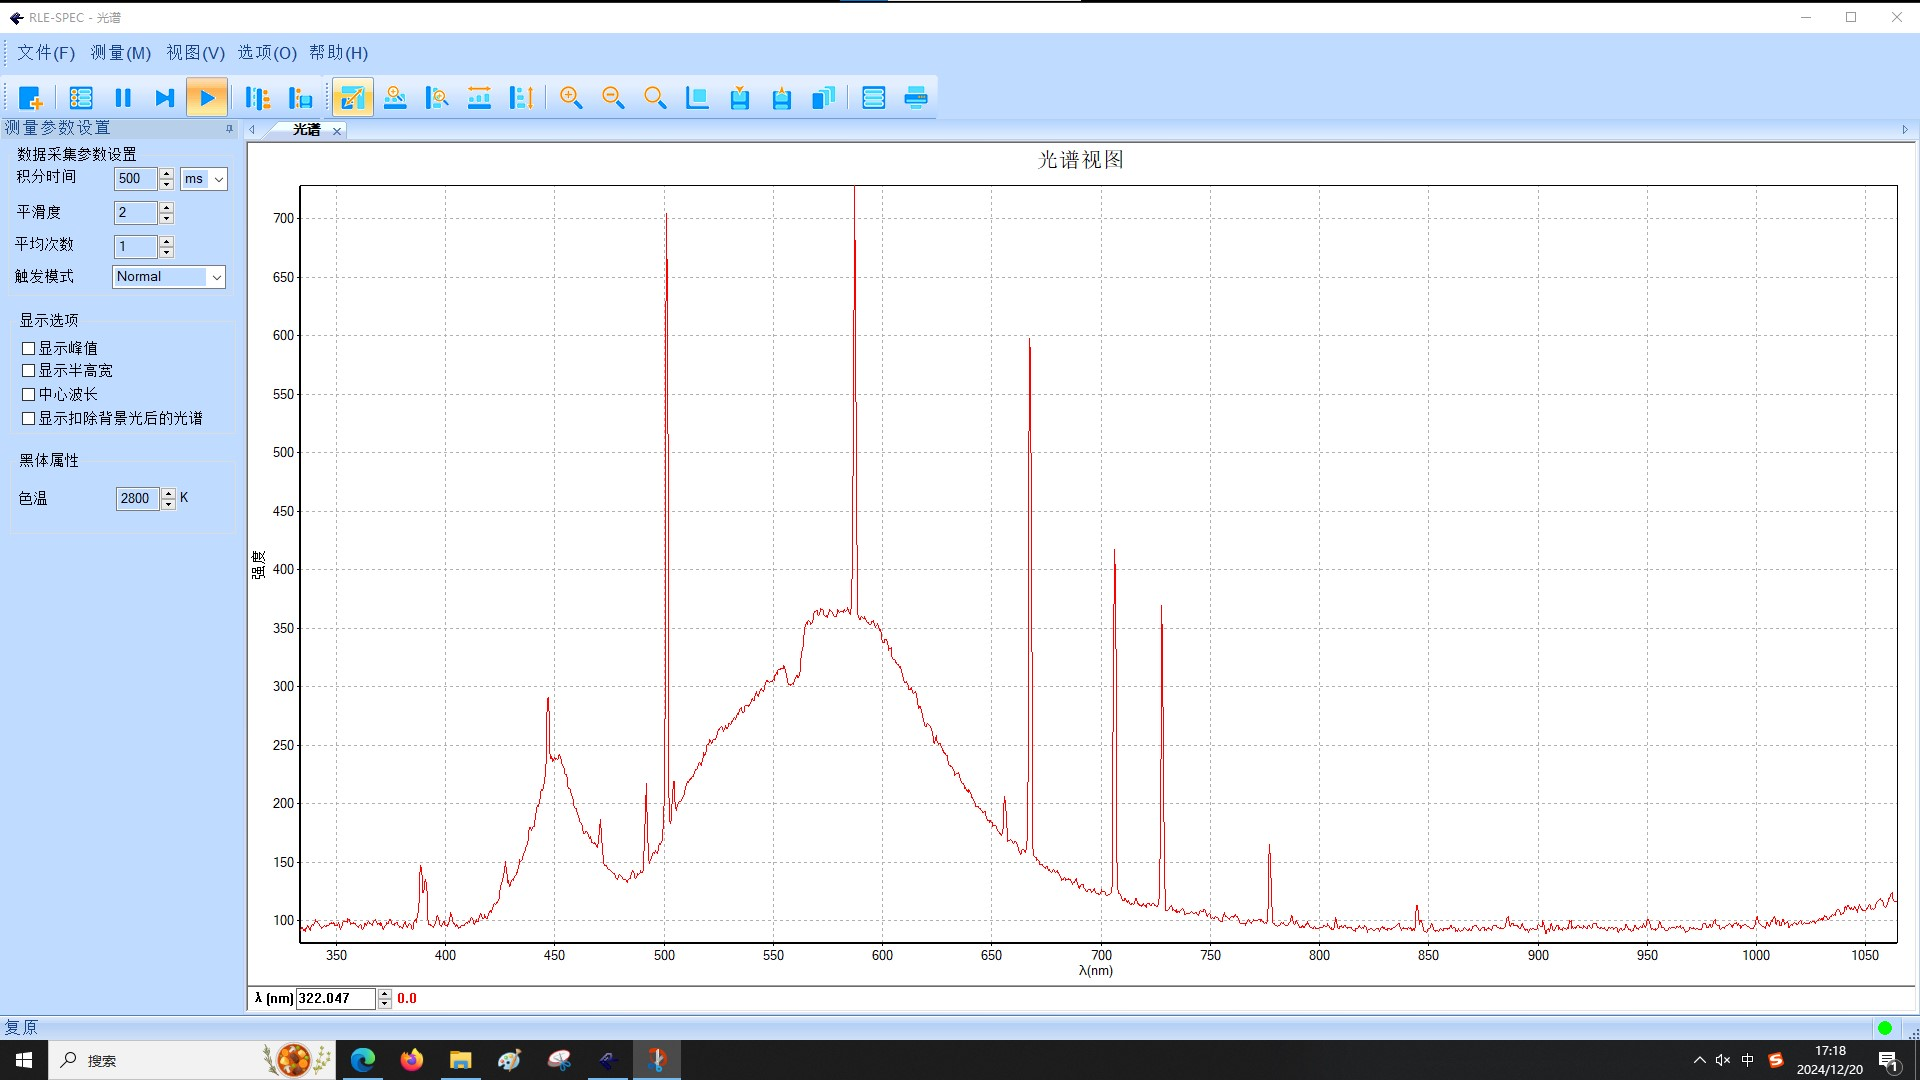
\includegraphics[width=0.6\linewidth]{images/APL1_2_exp3_He_O}
	\caption{原始数据展示}
	\label{fig:apl12exp3heo}
\end{figure}

\begin{figure}
	\centering
	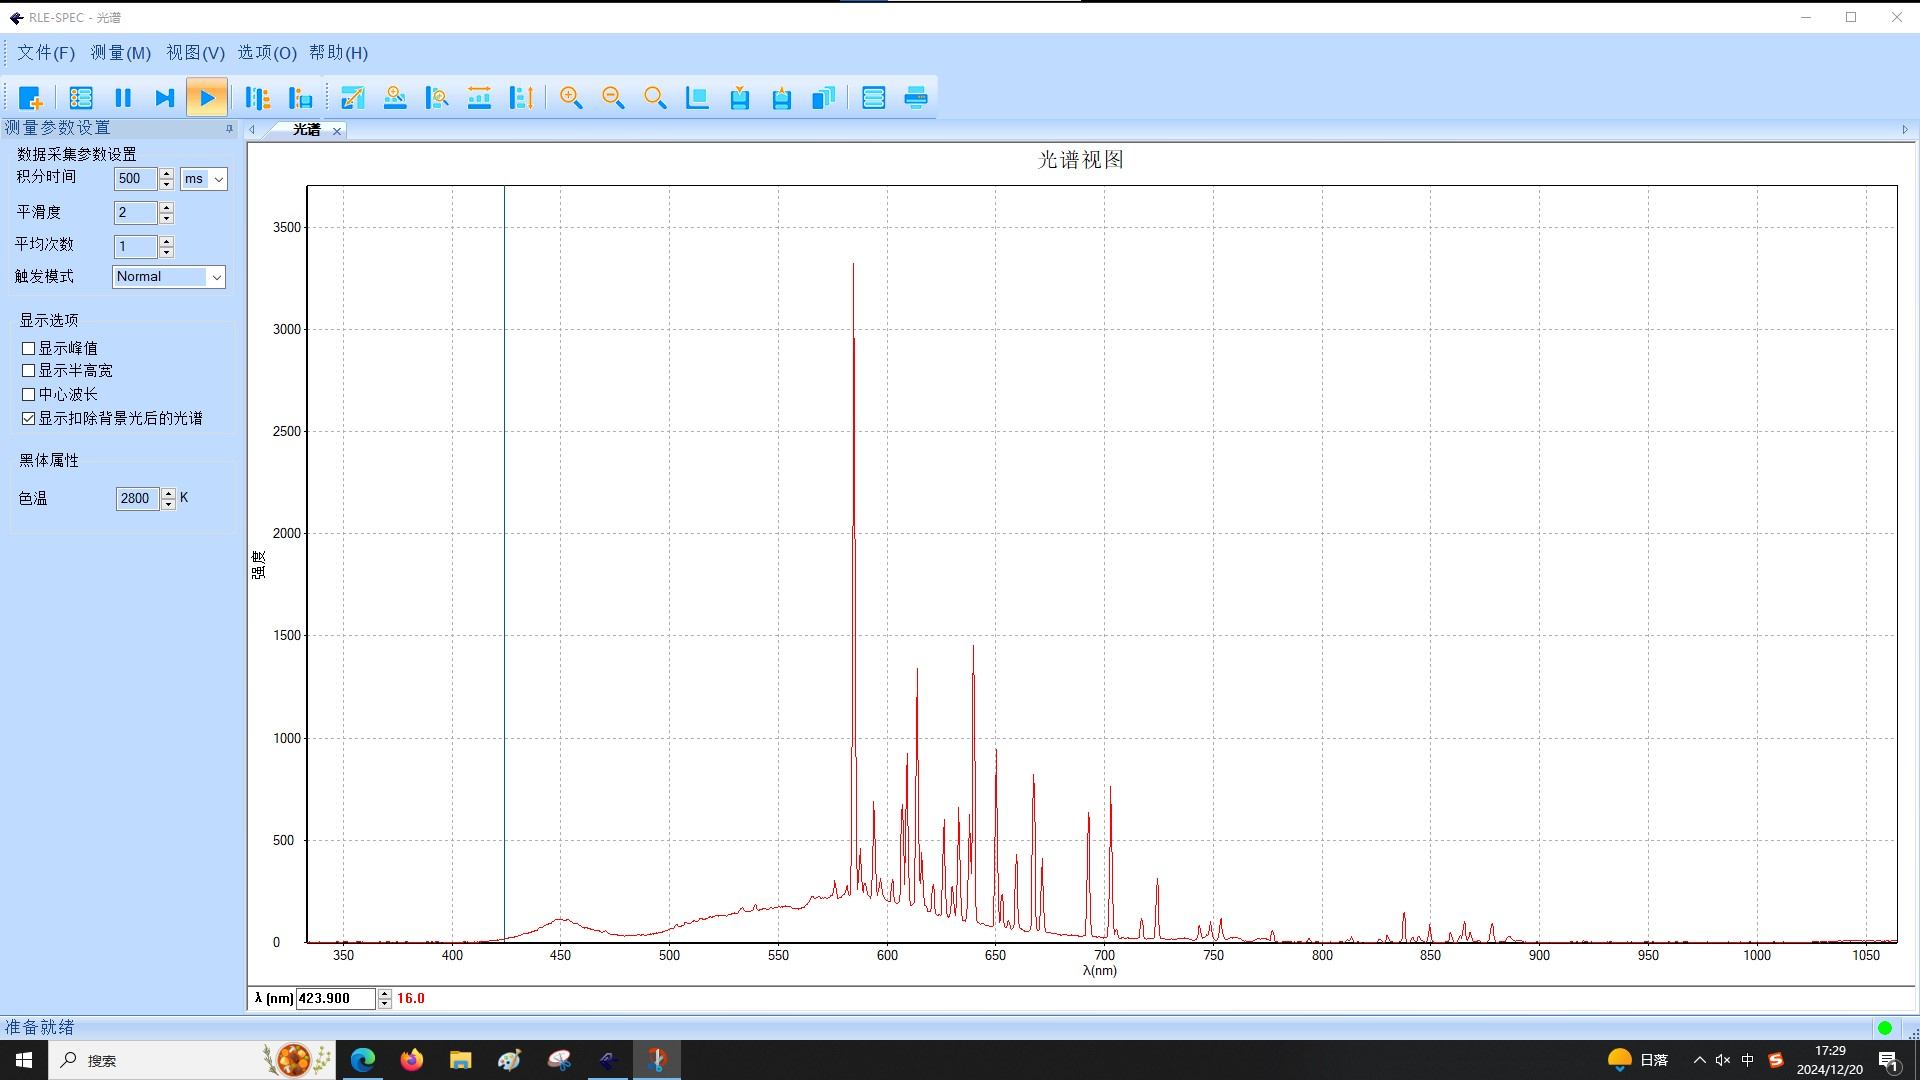
\includegraphics[width=0.6\linewidth]{images/APL1_2_exp3_Ne_O}
	\caption{原始数据展示}
	\label{fig:apl12exp3neo}
\end{figure}

\begin{figure}
	\centering
	\includegraphics[width=0.7\linewidth]{images/D2-OriginalData-1}
	\caption{原始数据记录}
	\label{fig:d2-originaldata-1}
\end{figure}

\begin{figure}
	\centering
	\includegraphics[width=0.7\linewidth]{images/D2-OriginalData-2}
	\caption{原始数据记录}
	\label{fig:d2-originaldata-2}
\end{figure}

%See the \textbf{Attachment} section for the clean of the experimental bench desktop (%\cref{}).

%Other raw data are shown in %\cref{}.


%%---------------------------------------------------------------------
%% 问题记录
%\subsection{Difficulties}
%\begin{enumerate}
%	\item 
%\end{enumerate}
%% ---